% !TEX root = ../main.tex
\section*{Results}\label{sec:results}

Here we present the main results of the work. These are the new efficient gradient-based training methods, and the hardness of classical simulation of the model. Firstly we define the model we use, and its connection to previously known quantum circuit families. In the next section, we discuss the efficient training of the model, firstly recalling a previously known gradient-based training method, using the $\MMD$ cost function, and then moving onto our new training methods using the Stein discrepancy and the Sinkhorn divergence in the following sections. We then discuss the Sinkhorn divergence complexity in detail, and further argue why it should be used, based on its connection to Total Variation distance. In the next section, we then prove the hardness results mentioned above; that many circuits encountered during gradient based training are hard to classically simulate. In the next section, we discuss the potential ability of quantum generative models to learn distributions which are intractable to classical models, and provide a framework to study these advantages.


\subsection*{Ising Born Machine}
Firstly, we define the model we use for distribution learning. A generic Born machine consists of a parameterised quantum circuit producing samples as a result of measurements, and a classical optimisation loop to train the model to learn a data distribution. The circuits we study have the following structure:
\begin{small}
\begin{align*}
    \Qcircuit @C=0.6em @R=0.8em {
    \lstick{\ket{0}}    & \gate{H}  & \multigate{3}{U_z(\boldsymbol\alpha)} & \gate{U_f(\Gamma_1, \Delta_1, \Sigma_1)}  & \meter &\cw & \rstick{x_1} \\
    \lstick{\ket{0}}    & \gate{H}  & \ghost{U_z(\boldsymbol\alpha)}        & \gate{U_f(\Gamma_2, \Delta_2, \Sigma_2)}  & \meter &\cw & \rstick{x_2} \\
    \cdots              &           &                                       & \cdots                                    & \cdots &    &  \\
    \lstick{\ket{0}}    & \gate{H}  & \ghost{U_z(\boldsymbol\alpha)}        & \gate{U_f(\Gamma_n, \Delta_n, \Sigma_n)}  & \meter &\cw & \rstick{x_n} 
    }
\end{align*}
\end{small}


\noindent where $x_i \in \{0, 1\}$ and the unitaries are defined by \eqref{diagonalunitary} and \eqref{finalmeasurementgate}, where $S_j$ indicates the subset of qubits on which each operator, $j$, is applied. A boldface parameter indicates a set of parameters, $\boldsymbol\alpha = \{\alpha_j\}$.
\begin{align}
  &U_z(\boldsymbol\alpha) \coloneqq  \prod_j U_z \left( \alpha_j, S_j \right) = \prod_j\exp \left( i \alpha_j \bigotimes_{k \in S_j} Z_k \right)\label{diagonalunitary}\\
    &U_f \left( \mathbf{\Gamma}, \mathbf{\Delta}, \mathbf{\Sigma} \right) \coloneqq \exp\left(i\sum\limits_{k=1}^n \Gamma_k X_k + \Delta_k Y_k +\Sigma_k Z_k\right)    \label{finalmeasurementgate}
\end{align}

\noindent The operators, $X_k, Y_k, Z_k$ are the standard Pauli operators acting on qubit $k$.
Restricting to the case $|S_j| \leq 2$ (since only single and two-qubit gates are required for universal quantum computation) the term in the exponential of \eqref{diagonalunitary} becomes exactly an Ising Hamiltonian:
\begin{align}
 \mathcal{H} \coloneqq i\sum\limits_{i<j} J_{ij}Z_iZ_j + i\sum\limits_{k=1}^n b_k Z_k \label{iqp_ising_hamiltonian}
 \end{align}


\noindent where we are dividing the diagonal unitary parameters,  $\boldsymbol{\alpha} = \{J_{ij}, b_k\}$,  into local terms which act only on qubit $k$, $\{b_k\}$, and coupling terms between two qubits $i$ and $j$, $\{J_{ij}\}$. We call the model an \textit{Ising} Born machine ($\IBM$).
A measurement on all qubits in the computational basis results in sample vectors, $\mathbf{x} \in \mathcal{X}^n$, where $\mathbf{x}$ is a binary vector of length $n$, and $\mathcal{X} = \{0, 1\}$. These samples are drawn from the following distribution, $p_{\boldsymbol\theta}(\mathbf{x})$, parameterised by a set of angles, $\boldsymbol\theta = \{\boldsymbol\alpha, \mathbf{\Gamma}, \mathbf{\Delta}, \mathbf{\Sigma}\}$:
\begin{align}
    p_{\boldsymbol\theta}(\mathbf{x}) \coloneqq \left|\bra{\mathbf{x}}U_f \left( \mathbf{\Gamma}, \mathbf{\Delta}, \mathbf{\Sigma} \right) U_z(\boldsymbol\alpha)\ket{+}^{\otimes n}\right|^2
\end{align}
We denote the above model and parameters by $\IBM(\boldsymbol\alpha, \mathbf{\Gamma}, \mathbf{\Delta}, \mathbf{\Sigma})$. We choose this structure in order to easily recover two more well known circuit classes, namely Instantaneous Quantum Polynomial Time\cite{shepherd_temporally_2009} ($\IQP$) circuits, and the shallowest depth ($p=1$) version of the Quantum Approximate Optimisation Algorithm\cite{farhi_quantum_2014}, ($\QAOA$). $\IQP$ circuits are named due to the commuting structure of the unitary $U_z$,  and $\QAOA$\cite{farhi_quantum_2014} was originally developed as an approximate version of the Quantum Adiabatic Algorithm\cite{farhi_quantum_2000}. Both of these classes of circuits, are known to demonstrate quantum supremacy to varying degrees\cite{bremner_classical_2011, bremner_average-case_2016, farhi_quantum_2016, bremner_achieving_2017}, which we will extend here, using the results of ref.\cite{fujii_commuting_2017}.

These classes can be recovered by setting the parameters of an $\IBM$ as follows:

%\begin{multline}
%    IBM\left(\{J_{ij}, b_{k}\}, \mathbf{\Gamma} \\ = \left\{\frac{\pi}{2\sqrt{2}}\right\}, \mathbf{0}, \mathbf{\Sigma}=  \left\{\frac{\pi}{2\sqrt{2}}\right\}\right) = \IQP(\{J_{ij}, b_{k}\})
%\end{multline}
\[
\begin{array}{lll}
\IQP(\{J_{ij}, b_{k}\}) =\\
\IBM\left(\{J_{ij}, b_{k}\}, \mathbf{\Gamma} = \left\{\frac{\pi}{2\sqrt{2}}\right\}, \mathbf{0}, \mathbf{\Sigma}=  \left\{\frac{\pi}{2\sqrt{2}}\right\}\right) 
\\{}\\
\QAOA_{p=1}(\{J_{ij}, b_{k}\}, \mathbf{\Gamma}) =
\\
\IBM\left(\{J_{ij}, b_{k}\}, \mathbf{\Gamma} = -\mathbf{\Gamma}, \mathbf{0} , \mathbf{0}\right)
\end{array}
\]

\noindent We choose the final gate before the computational basis measurement to be in the form of \eqref{finalmeasurementgate}, rather than the more common Euler decomposition of a single qubit gate decomposition found in the literature\cite{liu_differentiable_2018, du_expressive_2018}. This is chosen to make the classical simulation hardness results more apparent in our proofs.

\subsection*{Training the Ising Born Machine}


% \begin{figure*}[ht]
%     \centering
%     \includegraphics[width = 0.45\textwidth]{images/machinelearningmodel.pdf}
%     \caption{Illustration of generative modelling procedure.}
%     \label{fig:machinelearningmodel}
% \end{figure*}

\begin{figure*}[ht]
\centering
            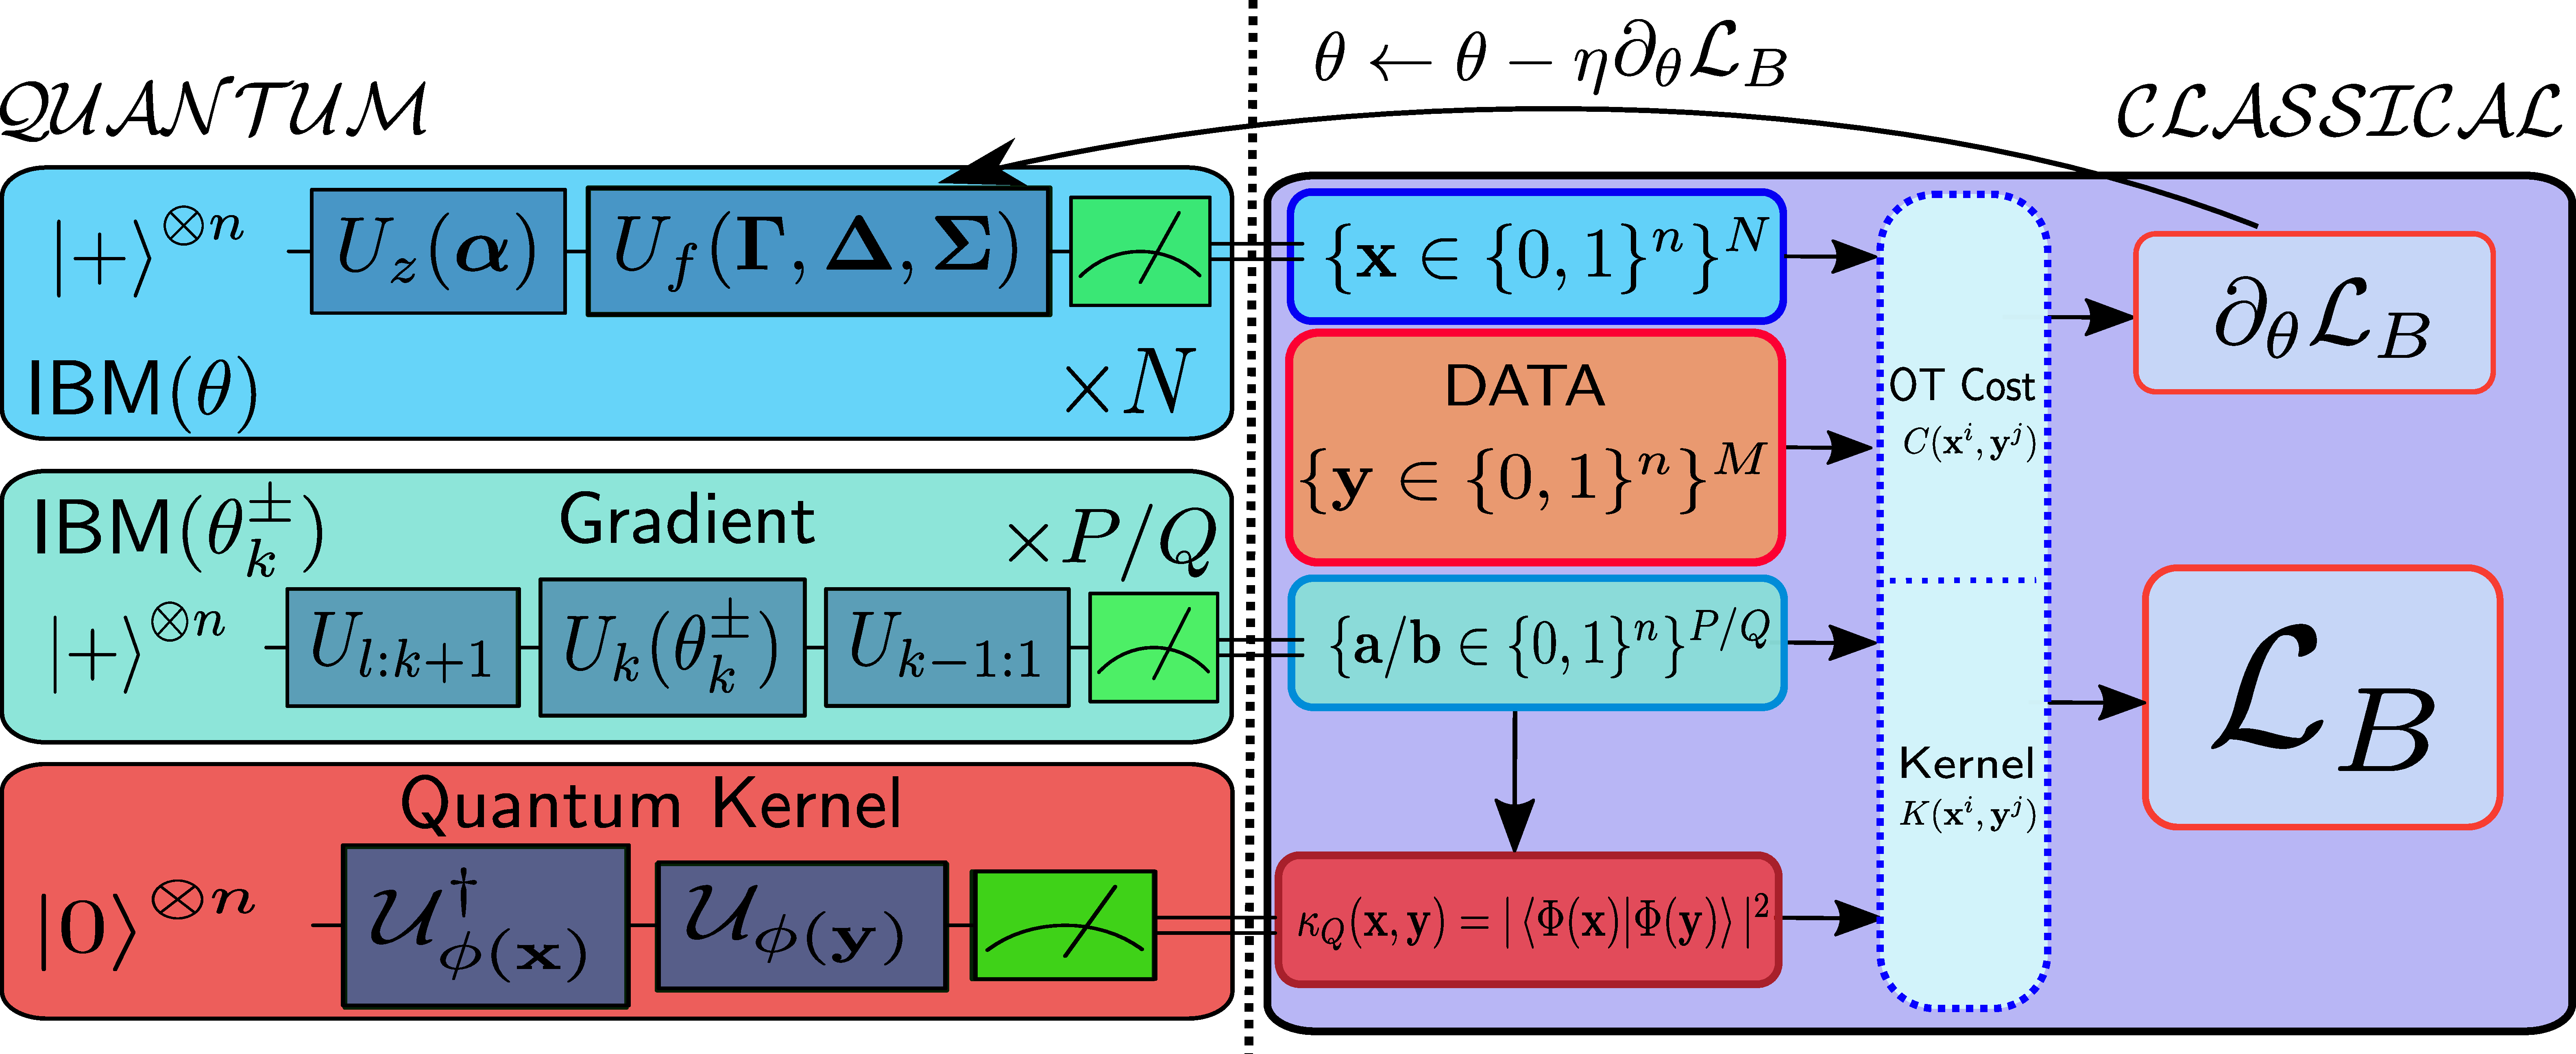
\includegraphics[width=\textwidth, height = 0.4\textwidth]{images/FIG_1a_pqc_npj.pdf}
            \caption{Hybrid training procedures we propose in this work. We have a quantum generator, along with auxiliary circuits used to compute the gradient of the various cost functions with respect to the parameters. Also, another quantum circuit can be run to evaluate the quantum kernel which is fed into the either the Stein discrepancy cost function, or the $\MMD$. For the Sinkhorn divergence, a cost function is evaluated instead.}\label{fig:ibmtraining}
\end{figure*}

Next, we introduce the alternative training methods we use which in fact are applicable to any generative model. The training procedure is a classical quantum hybrid, where the only quantum component is the model itself, and the rest of the computation is classical, which is as close to the capabilities of NISQ devices as possible. This can be seen in \figref{fig:ibmtraining}. The optimisation procedures we implement are stochastic gradient descents which use the following update rule for the parameters, $\theta_k$, for each epoch of training, $d$, $\theta^{d+1}_k \leftarrow \theta_k^{d} - \eta\, \partial_{\theta_k}\mathcal{L}_B$. The parameter $\eta$ is the learning rate, and controls the speed of the descent. The initial proposals to train BMs were gradient-free\cite{benedetti_generative_2019, leyton-ortega_robust_2019}, but these %tend to perform poorly in large parameter spaces and 
have shown to be outperformed by gradient methods for Born Machines\cite{liu_differentiable_2018, du_expressive_2018}. In this work, we advocate for increasing the classical computational power required in training to achieve better performance, rather than increasing the quantum resources, for example by adding extra ancillae\cite{du_expressive_2018} or adding costly and potentially unstable (quantum) adversaries\cite{zeng_learning_2018, lloyd_quantum_2018, dallaire-demers_quantum_2018}. 

For gradient-based methods, some \textit{cost function} or metric is required, $\mathcal{L}_B\left(p_{\boldsymbol\theta}(\mathbf{x}), \pi(\mathbf{y})\right)$ to compare between the Born Machine distribution, $p_{\boldsymbol\theta}(\mathbf{x})$, the data distribution, $\pi(\mathbf{y})$. Good cost functions will have several characteristics. They should be as efficient to compute as possible, both in terms of sample and computational complexity. They should also be powerful, in the sense that they are sensitive to differences between the two distributions. In this work, we will assess sensitivity by using %centre our ideas around 
the total variation ($\TV$) metric as a benchmark:
\begin{align}
    \TV(p_{\boldsymbol\theta}, \pi) \coloneqq \frac{1}{2}\sum_{\mathbf{x}}|p_{\boldsymbol\theta}(\mathbf{x}) - \pi(\mathbf{x})| \label{total_variation}
\end{align}

\noindent This is a particularly strong metric, in the sense that convergence in $\TV$ is one of the strongest notions of convergence in probability. The cost functions we use are typically easier to deal with than $\TV$, and we remark on their connections. One of the most common cost functions used to train generative models is the Kullback-Leibler ($\KL$) divergence. The $\KL$ divergence is also relatively strong, in the sense that it upper bounds $\TV$ through Pinsker's inequality. Unfortunately, this means it is difficult to compute in terms of sample complexity; neither its gradient, nor the $\KL$ divergence itself can be evaluated efficiently when training parameterised circuits \cite{liu_differentiable_2018}.

The first efficient gradient method to train Born machines was proposed by ref.\cite{liu_differentiable_2018}. 
%The key realisation is that the $\KL$ divergence is perhaps \textit{too strong} of a cost function, and we must settle for a weaker one. 
The idea is to use the \textit{maximum mean discrepancy} ($\MMD$) to define the cost function. We extend this methodology in two ways. The first is an improvement to the $\MMD$ itself, and the second is by introducing alternative cost functions. From the $\MMD$, the following cost function\cite{borgwardt_integrating_2006, gretton_kernel_2007} can be defined:
\begin{align}
   \mathcal{L}_{\MMD} & \coloneqq \underset{\substack{\mathbf{x} \sim p_{\boldsymbol\theta}\\ \mathbf{y} \sim p_{\boldsymbol\theta}}}{\mathbb{E}}(\kappa(\mathbf{x},\mathbf{y})) + \underset{\substack{\mathbf{x} \sim \pi \\\mathbf{y} \sim \pi }}{\mathbb{E}}(\kappa(\mathbf{x},\mathbf{y})) -\underset{\substack{\mathbf{x} \sim p_{\boldsymbol\theta}\\ \mathbf{y} \sim \pi}}{2\mathbb{E}}(\kappa(\mathbf{x},\mathbf{y})) \label{mmdexact}
\end{align}

\noindent The $\MMD$ has some very favourable properties; it is a metric on the space of probability distributions, and it is relatively easy to compute. The function, $\kappa$ in \eqref{mmdexact} is a \textit{kernel function}, a measure of similarity between points in the sample space $ \mathbf{x}\in\mathcal{X}^n$. A popular choice for this function is the Gaussian mixture kernel\cite{liu_differentiable_2018}:
\begin{align}
    \kappa_G(\mathbf{x}, \mathbf{y}) \coloneqq  \frac{1}{c}\sum_{i=1}^c\exp\left(-\frac{||\mathbf{x}-\mathbf{y}||^2_2}{2\sigma_i^2}\right) \label{gaussiankernel}
\end{align}

The parameters, $\sigma_i$, are \emph{bandwidths} which determine the scale at which the samples are compared, and $||\cdot||_2$ is the $\ell_2$ norm.

A key realisation of recent works\cite{havlicek_supervised_2019, schuld_supervised_2018} of how to gain near term advantages using quantum computers in QML is to explore \textit{quantum} kernels, which can be evaluated on a quantum computer. To gain such an advantage, these kernels should be difficult to compute on a classical device. To the best of our knowledge, we are the first to investigate the use of quantum kernels for generative modelling.

In particular, we will adopt the following kernel\cite{havlicek_supervised_2019} in which the samples are encoded in a particular quantum state, $\ket{\phi(\mathbf{x})}$, via a \textit{feature map}, $\phi:\mathbf{x}\rightarrow \ket{\phi({\mathbf{x}})}$ and the kernel is the inner product between different vectors:
\begin{align}
    \kappa_Q(\mathbf{x}, \mathbf{y}) \coloneqq  |\braket{\phi(\mathbf{x})|\phi(\mathbf{y})}|^2 \label{quantumkernel}
\end{align}

\noindent The inner product, \eqref{quantumkernel}, is evaluated on a quantum computer, and is conjectured to be hard to compute on a classical one\cite{havlicek_supervised_2019}, given only a classical description of the quantum states.  The state $\ket{\phi(\mathbf{x})}$ is produced with an encoding unitary on an initial state, $\ket{\phi(\mathbf{x})} = \mathcal{U}_{\phi(\mathbf{x})}\ket{0}^{\otimes n}$.

The next required ingredient is the gradient of the cost function. For the $\MMD$, the gradient with respect to the  $k^{\text{th}}$ parameter\cite{liu_differentiable_2018}, carried by the $k^{\text{th}}$ unitary gate, $U_k(\theta_k)$, is given by: 
\begin{multline}
    \frac{\partial \mathcal{L}_{\MMD}}{\partial \theta_k} =\underset{\substack{\mathbf{a} \sim p_{\theta_k}^-\\ \mathbf{x} \sim p_{\boldsymbol\theta}}}{2\mathbb{E}}(\kappa(\mathbf{a}, \mathbf{x}))- \underset{\substack{\mathbf{b} \sim p^+_{\theta_k}\\ \mathbf{x} \sim p_{\boldsymbol\theta}}}{2\mathbb{E}}(\kappa(\mathbf{b}, \mathbf{x}))  \\
    - \underset{\substack{\mathbf{a} \sim p^-_{\theta_k}\\ \mathbf{y} \sim \pi}}{2\mathbb{E}}(\kappa(\mathbf{a}, \mathbf{y}))  +\underset{\substack{\mathbf{b} \sim p^+_{\theta_k}\\ \mathbf{y} \sim \pi}}{2\mathbb{E}}(\kappa(\mathbf{b}, \mathbf{y}))\label{mmdgradient}
\end{multline}

\noindent where $p^{\pm}_{\theta_k}$ are generated by running the following auxiliary circuits\cite{mitarai_quantum_2018, schuld_evaluating_2018} \textit{for each} 
unitary gate, $U_k(\theta_k)$:

\begin{align}
\Qcircuit @C=0.5em @R=1em {
\lstick{\ket{0}^{\otimes n}} & \gate{H^{\otimes n}} & \gate{U_{l:k+1}}&\gate{U_k(\theta_k^{\pm})}&\gate{U_{k-1:1}} & \meter &\cw 
 }
\label{circuit:gradientplusminuscircuit}
\end{align}

\noindent 
where $\theta_k^{\pm}:=\theta_k \pm\pi/2$. 
%notation of the $k^{th}$ parameter by a factor of $\pm\pi/2$ only, relative to the original parameterised circuit. 
The gradients of the cost functions which we introduce next 
will also include the parameter-shifted circuits in \eqref{circuit:gradientplusminuscircuit}. For more details on kernel methods and the $\MMD$, see \appref{supp_matt:kernelmethods_mmd}.


\begin{figure*}[t!]
 %   \centering
     \begin{subfigure}[t]{0.31\textwidth}
  %   \centering
    %     \includegraphics[width=\textwidth, height = 0.9\textwidth]{images/TV_4_qubits_mmd_kernel_comp_lr_Average_samples_500_batch_250.pdf}
         \begin{tikzpicture}
  \node (img)  {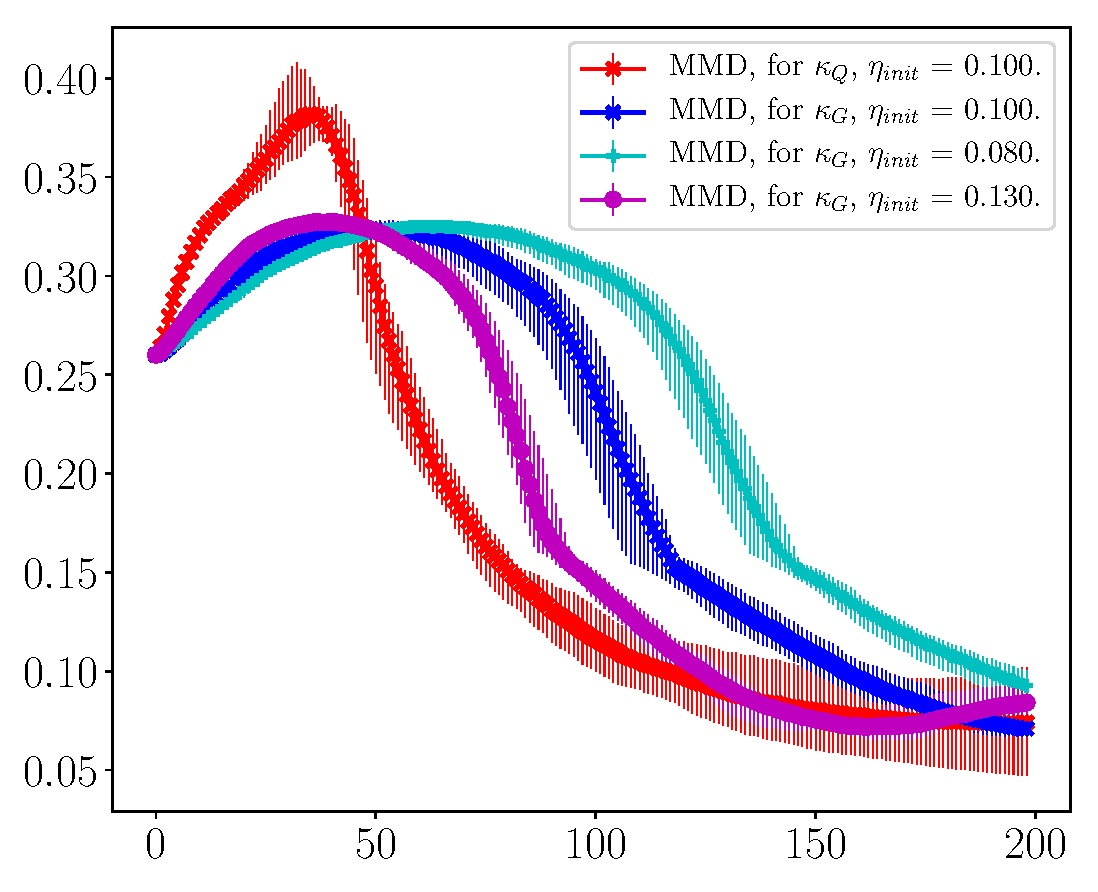
\includegraphics[width=0.95\textwidth, height = 0.8\textwidth]{images/FIG_2a_TV_4_qubits_mmd_kernel_comp_lr_Average_samples_500_batch_250_TAKE_two.pdf}};
  \node[below=of img, node distance=0cm, yshift=1.35cm,font=\color{black}] {epochs};
  \node[left=of img, node distance=0cm, rotate=90, anchor=center,yshift=-0.95cm,font=\color{black}] {$\TV$};
\end{tikzpicture}
        \caption{}
        \label{subfig:tv_4_qubits_mmd_gaussian_v_quantum}
    \end{subfigure}
    \begin{subfigure}[t]{0.31\textwidth}
   %  \centering
        % \includegraphics[width=\textwidth, height = 0.8\textwidth]{images/probs_4_qubits_mmd_kernel_comp_lr_0_1_AVG_samples_500_batch_250.pdf}
         \begin{tikzpicture}
  \node (img)  {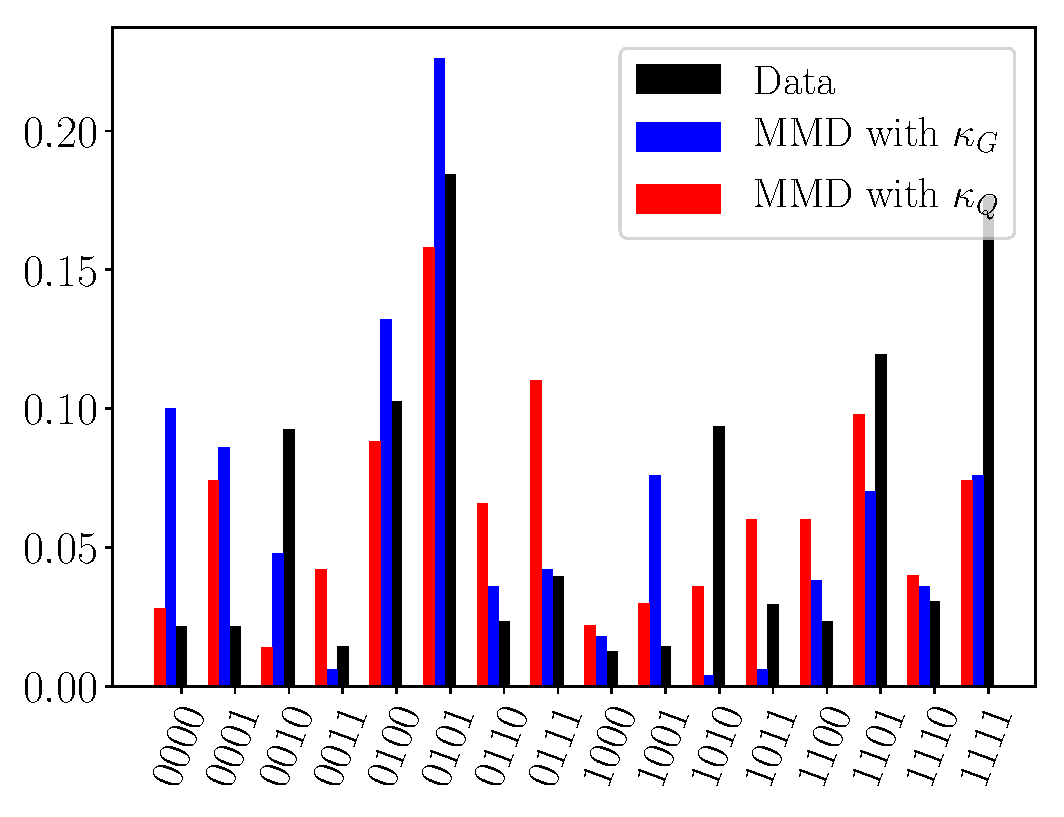
\includegraphics[width=\textwidth, height = 0.8\textwidth]{images/FIG_2b_probs_4_qubits_mmd_kernel_comp_lr_0_1_AVG_samples_500_batch_250.pdf}};
  \node[below=of img, node distance=0cm, yshift=1.29cm,font=\color{black}] {outcomes};
  \node[left=of img, node distance=0cm, rotate=90, anchor=center,yshift=-0.95cm,font=\color{black}] {probability};
\end{tikzpicture}
        \caption{}
        \label{subfig:probs_4_qubits_mmd_gaussian_v_quantum}
    \end{subfigure}
    ~ 
    \begin{subfigure}[t]{0.31\textwidth}
    % \centering
        % \includegraphics[width=\textwidth, height = 0.8\textwidth]{images/MMD_4_qubits_mmd_kernel_comp_Average_samples_500_batch_250.pdf}
         \begin{tikzpicture}
  \node (img)  {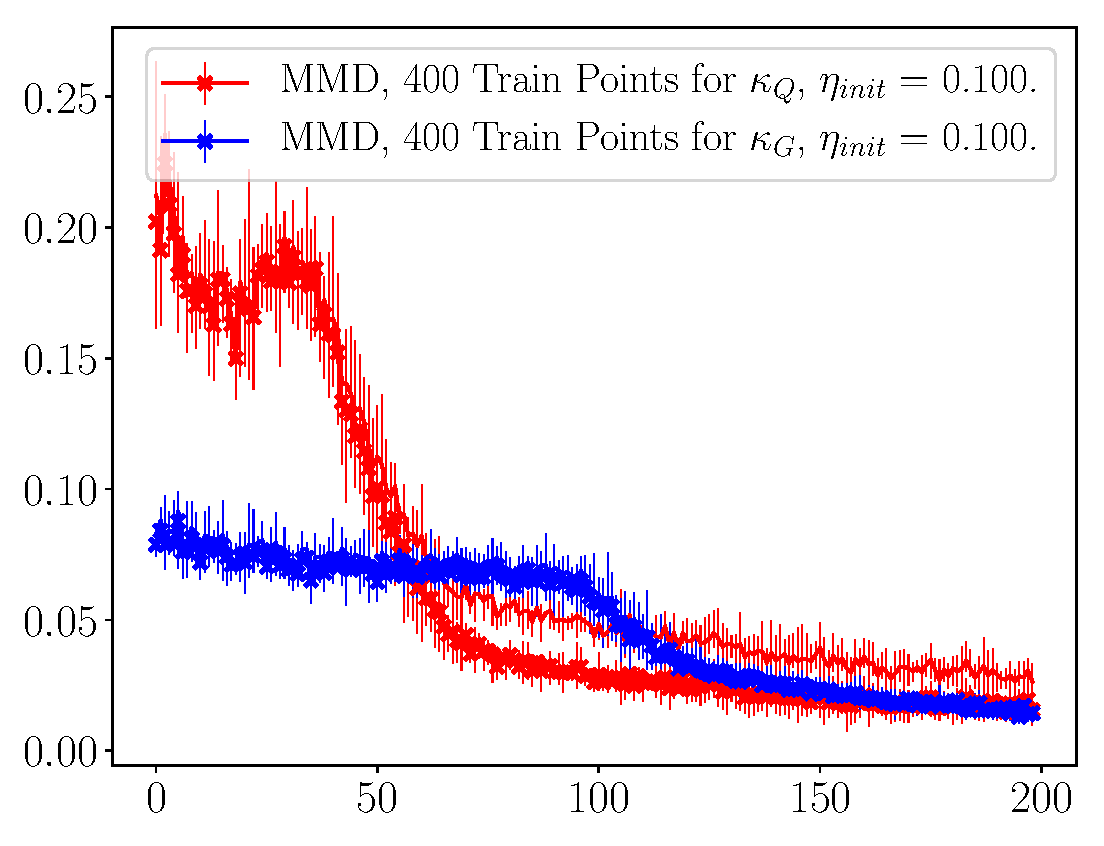
\includegraphics[width=\textwidth, height = 0.8\textwidth]{images/FIG_2c_MMD_4_qubits_mmd_kernel_comp_Average_samples_500_batch_250.pdf}};
  \node[below=of img, node distance=0cm, yshift=1.35cm,font=\color{black}] {epochs};
  \node[left=of img, node distance=0cm, rotate=90, anchor=center,yshift=-0.95cm,font=\color{black}] {$\MMD$ loss $\mathcal{L}_{\MMD}$};
\end{tikzpicture}
        \caption{}
        \label{subfig:mmd_kernel_comp_4_qubits}
    \end{subfigure}
\caption{
Performance of quantum $\kappa_Q$ [\crule[red]{0.2cm}{0.2cm}] vs.\@ Gaussian kernel,  
$\kappa_G$ [\crule[blue]{0.2cm}{0.2cm}] (with $\eta_{\mathsf{init}} = 0.1$) for 4 qubits. 
To train, we sample from the $\IBM$ and the data $500$ times and use a minibatch size of $250$. 
One epoch is one complete update of all parameters according to gradient descent. Error bars represent maximum, minimum and mean values achieved over 5 independent training runs, with the same initial conditions on the same data samples. (a) $\TV$ Difference achieved with both kernel methods during training. With the quantum kernel, a lower value of $\TV$ can be achieved than with a Gaussian kernel. Increasing the learning rate speeds up convergence, but still cannot achieved the same minimum $\TV$ (b) Final learned probabilities with $\eta_{\mathsf{init}} = 0.1$ using the Adam optimiser. (c) $\MMD$ computed using $400$ samples as training points, $100$ as test points, independent of the training data. $\MMD$ is seen to converge faster with the quantum kernel, although it appears to have a higher generalisation error.
\label{fig:QvGkernel4}
} 
\end{figure*}

% \begin{figure*}
%     \centering
%     \begin{subfigure}[t]{0.31\textwidth}
%         \includegraphics[width=\textwidth, height = 0.9\textwidth]{images/TV_4_qubits_mmd_kernel_comp_lr_Average_samples_500_batch_250.pdf}
%         \caption{}
%         \label{subfig:tv_4_qubits_mmd_gaussian_v_quantum}
%     \end{subfigure}
%     ~ 
%     \begin{subfigure}[t]{0.31\textwidth}
%         \includegraphics[width=\textwidth, height = 0.9\textwidth]{images/probs_4_qubits_mmd_kernel_comp_lr_0_1_AVG_samples_500_batch_250.pdf}
%         \caption{}
%         \label{fig:probs_4_qubits_mmd_gaussian_v_quantum}
%     \end{subfigure}
%     ~ 
%     \begin{subfigure}[t]{0.31\textwidth}
%         \includegraphics[width=\textwidth, height = 0.9\textwidth]{images/MMD_4_qubits_mmd_kernel_comp_Average_samples_500_batch_250.pdf}
%         \caption{}
%         \label{subfig:mmd_kernel_comp_4_qubits}
%     \end{subfigure}
%     \caption{Quantum vs. Gaussian kernel for 4 qubits. $500$ samples from $\IBM$ and Data, Batch Size $ = 250$. (a) $\TV$ Difference between $\kappa_G$ [\crule[blue]{0.2cm}{0.2cm}] and $\kappa_Q$ [\crule[red]{0.2cm}{0.2cm}]. (b) Final learned probabilities using $\kappa_G$ [\crule[blue]{0.2cm}{0.2cm}] and $\kappa_Q$ [\crule[red]{0.2cm}{0.2cm}] with $\eta_{\mathsf{init}} = 0.1$. (c)$\MMD$ using $\kappa_G$ [\crule[blue]{0.2cm}{0.2cm}] vs. $\kappa_Q$ [\crule[red]{0.2cm}{0.2cm}] on $400$ training data points, $100$ test data points.}\label{fig:QvGkernel4}
% \end{figure*}

\subsection*{Stein Discrepancy Training}\label{ssec:steintrainingofibm}
So far, we have only proposed a change of kernel in the $\MMD$ method to train 
$\IBM$s. We are now going to consider changing the cost function altogether. We endeavour to find such costs which are efficient to compute for quantum models, yet stronger than $\MMD$. 
The first cost we propose is called the \textit{Stein discrepancy} ($\SD$). $\SD$ has become popular for goodness-of-fit tests\cite{liu_kernelized_2016}, i.e.\@ testing whether samples come from a particular distribution or not, as opposed to the $\MMD$, which is typically used for kernel two-sample tests\cite{gretton_kernel_2007}. 
We use the discrete version of the Stein discrepancy\cite{yang_goodness--fit_2018} here, since in its original form\cite{liu_kernelized_2016}, it only caters for the case where the distributions are supported over a \textit{continuous} space. The discretisation is necessary since the $\IBM$ outputs binary strings and so the standard gradient w.r.t.\@ a sample, $\mathbf{x}$, $\nabla_{\mathbf{x}}$, is undefined. As such, we need to use a discrete `shift' operator instead, $\Delta_{\mathbf{x}}$; an operator defined by $[\Delta_\mathbf{x}f(\mathbf{x})]_i \coloneqq f(\mathbf{x}) - f(\neg_i\mathbf{x})$ for a function $f$,
where $\neg_i$ flips the $i^{th}$ element of the binary vector $\mathbf{x}$. Fortunately, the discretisation procedure is relatively straightforward (necessary definitions and proofs in \appref{supp_matt:stein_discrepenancy}).
The discrepancy is derived\cite{liu_kernelized_2016, gorham_measuring_2015} from the (discrete) Stein Identity\cite{yang_goodness--fit_2018}, given by:
\begin{align}
    \underset{\mathbf{x}\sim \pi}{\mathbb{E}}[\mathcal{A}_\pi \phi(\mathbf{x})]= \mathbb{E}_{\mathbf{x} \sim \pi}\left[\mathbf{s}_\pi(\mathbf{x})\phi(\mathbf{x}) - \Delta_{\mathbf{x}} \phi(\mathbf{x})\right] = 0 
    \label{complexdiscretesteinidentity}
\end{align}

\noindent where $\underset{\mathbf{x}\sim \pi}{\mathbb{E}}$ denotes the expectation value over the distribution, $\pi$. This holds for any function $\phi: \mathcal{X}^n\rightarrow \mathbb{C}$, and a probability mass function $\pi$ on $\mathcal{X}^n$. The function, $s_\pi(\mathbf{x}) = \Delta_\mathbf{x}\log(\pi(\mathbf{x}))$ is the \textit{Stein score} function of the distribution $\pi$, and $\mathcal{A}_\pi$ is a so-called \textit{Stein operator} of $\pi$. The functions that obey, \eqref{complexdiscretesteinidentity}, are said to be in the \textit{Stein class} of the distribution $\pi$.  Now, the $\SD$ cost function can be written in a kernelised form\cite{liu_kernelized_2016, yang_goodness--fit_2018}, similarly to the $\MMD$:
\begin{align}
    \mathcal{L}_{\SD}(p_{\boldsymbol\theta}, \pi)\coloneqq \mathbb{E}_{\mathbf{x}, \mathbf{y}\sim p_{\boldsymbol\theta}}\left[\kappa_\pi(\mathbf{x}, \mathbf{y})\right]\label{steindiscrepancybornmachine}
\end{align}
\begin{multline}
    \kappa_\pi(\mathbf{x}, \mathbf{y}) \coloneqq s_\pi(\mathbf{x})^T\kappa(\mathbf{x}, \mathbf{y})s_\pi(\mathbf{y}) -s_\pi(\mathbf{x})^T\Delta_{\mathbf{y}}^*\kappa(\mathbf{x}, \mathbf{y}) \\
    - \Delta_{\mathbf{x}}^*\kappa(\mathbf{x}, \mathbf{y})^Ts_\pi(\mathbf{y}) + \tr(\Delta_{\mathbf{x}, \mathbf{y}}^*\kappa(\mathbf{x}, \mathbf{y})) \label{weightedkernelbornmachine}
\end{multline}
$\kappa_\pi$ is the \textit{Stein kernel}, and $\kappa$ is a usual positive semi-definite kernel. $\Delta_{\mathbf{x}}^*$ is a conjugate version of the operator $\Delta_{\mathbf{x}}$, but for our purposes, the behaviour of both $\Delta_{\mathbf{x}}^*$ and $\Delta_{\mathbf{x}}$ are identical. For completeness, we define it in generality in \appref{supp_matt:stein_discrepenancy}.

Just as above, the gradient (derived in \appref{supp_matt:stein_discrepenancy}) of $\mathcal{L}_{\SD}$ with respect to the parameter, $\theta_k$, is given by:
\begin{multline}
    \frac{\partial \mathcal{L}_{\SD}}{\partial \theta_k} = \underset{\substack{\mathbf{x} \sim p^-_{\boldsymbol\theta} \\ \mathbf{y}\sim p_{\boldsymbol\theta}}}{\mathbb{E}}[\kappa_\pi(\mathbf{x}, \mathbf{y})] - \underset{\substack{\mathbf{x} \sim p^+_{\boldsymbol\theta} \\ \mathbf{y}\sim p_{\boldsymbol\theta}}}{\mathbb{E}}[\kappa_\pi(\mathbf{x}, \mathbf{y})]\\ +\underset{\substack{\mathbf{x} \sim p_{\boldsymbol\theta}\\ \mathbf{y}\sim p^-_{\boldsymbol\theta}}}{\mathbb{E}}[\kappa_\pi(\mathbf{x}, \mathbf{y})] - \underset{\substack{\mathbf{x} \sim p_{\boldsymbol\theta} \\ \mathbf{y}\sim p^+_{\boldsymbol\theta}}}{\mathbb{E}}[\kappa_\pi(\mathbf{x}, \mathbf{y})] \label{steingradient}
\end{multline}

\noindent Complementary to this, we show that almost every term in \eqref{steindiscrepancybornmachine} and \eqref{steingradient} can be computed efficiently, even when using the quantum kernel in \eqref{quantumkernel}, $\kappa_Q$, in \eqref{weightedkernelbornmachine}. This is, with the exception of the score function $s_\pi$ with respect to the data distribution. This is because the score has an explicit dependence on the data distribution, $\pi$. If we are given oracle access to the probabilities, $\pi(\mathbf{y})$, then there is no issue and $\SD$ will be computable. Unfortunately, in any practical application this will not be the case. To deal with such a scenario, we give two approaches to approximate the score via samples from $\pi$. The first of these we call the `Identity' method since it inverts Stein's identity\cite{li_gradient_2018}. We refer to the second as the `Spectral' method since it uses a spectral decomposition\cite{shi_spectral_2018} of a kernel to approximate the score. We will only use the Spectral method in training the $\IBM$ in the numerical results \figref{fig:MMDvSinkvStein3}, since the Identity method does not give an immediate out-of-sample method to compute the score. Details of these methods can be found in \appref{supp_matt:stein_discrepenancy}. Notice that even with the difficulty in computing the score, the $\SD$ is still more suitable than the $\KL$ divergence to train these models, since the latter requires computing the \textit{circuit} probabilities, $p_{\boldsymbol\theta}(\mathbf{x})$, which is in general intractable, and so could not be computed for \textit{any} dataset. 


\subsection*{Sinkhorn Divergence Training \label{ssec:sinkhorntrainingofibm}}
The second cost function we consider is the so-called \textit{Sinkhorn Divergence} ($\SH$). This is a relatively new method to compare probability distributions \cite{ramdas_wasserstein_2015, genevay_learning_2017, feydy_interpolating_2018} , defined by the following:
\begin{align}
    \mathcal{L}_{\SH}^\epsilon(p_{\boldsymbol\theta}, \pi) \coloneqq \OT^c_\epsilon(p_{\boldsymbol\theta}, \pi) - \frac{1}{2} \OT^c_\epsilon(p_{\boldsymbol\theta}, p_{\boldsymbol\theta}) -\frac{1}{2}\OT^c_\epsilon(\pi, \pi) \label{sinkhorndivergence}
\end{align}
\begin{multline}
    \OT^c_\epsilon(p_{\boldsymbol\theta}, \pi) \coloneqq \\
      \min\limits_{U \in \mathcal{U}(p_{\boldsymbol\theta}, \pi)}\left(\sum\limits_{\substack{(\mathbf{x}, \mathbf{y})\\ \in \mathcal{X}^d\times\mathcal{Y}^d}} c(\mathbf{x}, \mathbf{y})U(\mathbf{x}, \mathbf{y}) + \epsilon \KL(U|p_{\boldsymbol\theta}\otimes \pi)\right) \label{wassersteinregularised}
\end{multline}

\noindent where $\epsilon \geq 0 $ is a regularisation parameter, and $\mathcal{U}(p_{\boldsymbol\theta}, \pi)$ is the set of all \textit{couplings} between $p_{\boldsymbol\theta}$ and $\pi$, i.e.\@ the set of all joint distributions, whose marginals with respect to $\mathbf{x}, \mathbf{y}$ are $p_{\boldsymbol\theta}(\mathbf{x}), \pi(\mathbf{y})$ respectively. 
The above cost function, $\mathcal{L}_{\SH}^\epsilon$, is particularly favourable as a candidate because of its relationship to the theory of \textit{optimal transport}\cite{villani_optimal_2009} ($\OT$),  an old method to compare probability distributions. It has become a major tool used to train models in the classical domain, for example with GANs\cite{arjovsky_wasserstein_2017} through a restriction of optimal transport called the Wasserstein metric, which is derived from
$\OT$, when the cost, $c$, is chosen to be a metric on the space of $\mathcal{X}^n$.

We would like to use $\OT$ \textit{itself} to train generative models, due to its metric properties. Unfortunately, $\OT$ has high computational cost and exponential sample complexity\cite{dudley_speed_1969}. For this reason, the Sinkhorn divergence was proposed in refs. \cite{ramdas_wasserstein_2015, genevay_learning_2017, feydy_interpolating_2018} to \textit{interpolate} between $\OT$ and the $\MMD$ as a function of the regularisation parameter, $\epsilon$ in \eqref{wassersteinregularised}. In particular, for the two extreme values for $\epsilon$, we recover\cite{ramdas_wasserstein_2015} both unregularised $\OT$, and the $\MMD$:
\begin{align}
&\epsilon \rightarrow 0 :\mathcal{L}_{\SH}^0(p_{\boldsymbol\theta}, \pi)\rightarrow \OT_0^c(p_{\boldsymbol\theta}, \pi)\\
&\epsilon \rightarrow \infty:
\mathcal{L}_{\SH}^\epsilon(p_{\boldsymbol\theta}, \pi) \rightarrow  \MMD(p_{\boldsymbol\theta}, \pi) : \kappa(\mathbf{x}, \mathbf{y}) = -c(\mathbf{x}, \mathbf{y})
\end{align}
Now, as before, we need a gradient of the $\mathcal{L}_{\SH}$ with respect to the parameters, given by:
\begin{align}
    \frac{\partial \mathcal{L}_{\SH}^\epsilon(p_{\boldsymbol\theta}, \pi)}{\partial \theta_k} 
    & = \underset{\substack{\mathbf{x} \sim p_{\theta_k^-} }}{\mathbb{E}}[\varphi(\mathbf{x})] 
    -\underset{\substack{\mathbf{x} \sim p_{\theta_k^+}  }}{\mathbb{E}}[\varphi(\mathbf{x})] \label{sinkhorngradient}
\end{align}

Where $\varphi(\mathbf{x})$ is a function which depends on the optimal solutions found to the regularised $\OT$ problem in \eqref{wassersteinregularised}. See \appref{supp_matt:sinkhorn} for more details on the Sinkhorn divergence, and its gradient.

% \end{onecolumn}
\subsubsection*{Sinkhorn Complexity}
The sample complexity of the Sinkhorn Divergence is of crucial interest to us; we claim that the $\TV$ and the $\KL$ are not suitable directly as cost functions due to the difficulty of computing the outcome probabilities of quantum circuits efficiently. We now motivate why the $\MMD$ is a weak cost function, and why the Sinkhorn Divergence should be used as an alternative. This will depend critically on the regularisation parameter $\epsilon$, which allows a smooth interpolation between the $\OT$ metric and the $\MMD$ one. 

Firstly, we will address the computability of $\mathcal{L}_{\SH}$ and we find, due to the results of ref. \cite{genevay_sample_2018}, a somewhat `optimal' value for $\epsilon$, such that the sample complexity of $\mathcal{L}_{\SH}$ looks efficient. Specifically, the mean error between $\mathcal{L}_{\SH}$ and its approximation $\hat{\mathcal{L}}_{\SH}$, computed using $M$ samples, scales as:
\begin{align}
     &\mathbb{E}|\mathcal{L}_{\SH}^\epsilon - \hat{\mathcal{L}}_{\SH}^\epsilon| \leq \frac{3K}{\sqrt{M}}\left(1+e^{\left(2\frac{n^2+n}{\epsilon}\right)}\right)\mathcal{O}\left(1+\frac{1}{\epsilon^{\lfloor n/2\rfloor}}\right)
\end{align}

\noindent Hence, by choosing $\epsilon = \mathcal{O}(n^{2})$, we get:
\begin{align}
     &\mathbb{E}|\mathcal{L}_{\SH}^{\mathcal{O}(n^{2})} - \hat{\mathcal{L}}_{\SH}^{ \mathcal{O}(n^{2})}| =~ \mathcal{O}\left(\frac{1}{\sqrt{M}}\right) \label{sinkhorn_expectation_sample_chosen_MAIN}
\end{align}

\noindent which is the same sample complexity as the $\MMD$\cite{sriperumbudur_integral_2009}, but exponentially better than that of unregularised optimal transport, which scales as $\mathcal{O}\left(1/{M}^{1/n}\right)$\cite{dudley_speed_1969}. A similar result can be derived using a concentration bound\cite{genevay_sample_2018}, such that with probability $1-\delta$, 
\begin{align}
    |\mathcal{L}_{\SH}^{O(n^{2})}  - \hat{\mathcal{L}}_{\SH}^{O(n^{2})} | 
    = \mathcal{O}\left(\frac{1}{\sqrt{M}}\log(1/\delta)^{1/2}\right) \label{sinkhornborn_samplecomplexity_choosed_MAIN}
\end{align}

\noindent Where we have chosen the same scaling for $\epsilon$ as in \eqref{sinkhorn_expectation_sample_chosen_MAIN}. Therefore, we can choose an optimal theoretical value for the regularisation, such that $\mathcal{L}_{\SH}$ is sufficiently far from $\OT$ to be efficiently computable, but perhaps still retains some of its favourable properties. It is likely in practice however, that a much lower value of $\epsilon$ could be chosen without a blow up in sample complexity\cite{genevay_learning_2017,  genevay_sample_2018}. See \appref{supp_matt:sinkhorn} for derivations of these two results.

Secondly, we can relate the $\mathcal{L}_{\SH}$ to unregularised $\OT$ and $\TV$ via a sequence of inequalities. We have mentioned that the $\MMD$ is weak, meaning it provides a \textit{lower} bound on $\TV$ in the following way\cite{sriperumbudur_integral_2009}:
\begin{align}
    \TV(p_{\boldsymbol\theta}, \pi) \geq \frac{\sqrt{\MMD(p_{\boldsymbol\theta}, \pi)}}{\sqrt{C}}
\end{align}


\noindent if $C := \sup_{\mathbf{x} \in \mathcal{X}^n} \kappa(\mathbf{x}, \mathbf{x}) < \infty$. 

Note that for the two kernels introduced earlier:
\begin{align}
\kappa_G(\mathbf{x}, \mathbf{x}) &= \frac{1}{c}\sum\limits_{i=1}^c e^{-\frac{1}{2\sigma_i}|\mathbf{x} - \mathbf{x}|^2} =\frac{1}{c}(c) = 1\\
\kappa_Q(\mathbf{x}, \mathbf{x}) &= |\braket{\phi(\mathbf{x})|\phi(\mathbf{x})}|^2 = |\braket{0|0}^{\otimes n}|^2 = 1 %\forall \mathbf{x}
\end{align}
hence $C = 1$ and the lower bound is immediate. 

In contrast, the Wasserstein metric (unregularised $\OT$) provides an \textit{upper} bound on $\TV$, and hence we would expect it to be stronger then the $\MMD$ due to the following inequality on a discrete sample space \cite{gibbs_choosing_2002}:
\begin{align}
    d_{min} \TV(p_{\boldsymbol\theta}, \pi) \leq \OT^d_0(p_{\boldsymbol\theta}, \pi) \leq \text{diam}(\mathcal{X})\TV(p_{\boldsymbol\theta}, \pi) \label{tv_wasserstein_inequality}
\end{align}
where $\text{diam}(\mathcal{X}^n) = \max\{d(\mathbf{x}, \mathbf{y}), \mathbf{x}, \mathbf{y} \in \mathcal{X}^n\}$, $ d_{min} = \min_{x\neq y}d(\mathbf{x}, \mathbf{y})$, and $d(\mathbf{x}, \mathbf{y})$ is the metric on the space, $\mathcal{X}^n$. This arises by choosing $c = d$ and $\epsilon = 0$ in the above \eqref{wassersteinregularised}. If, for instance, we were to choose $d(\mathbf{x}, \mathbf{y})$ to be the $\ell_1$ metric between the binary vectors of length $d$(a.k.a.\@ the  Hamming distance), then we get that $ d_{min} = 1, \text{diam}(\mathcal{X}) = n$, and so:
\begin{align}
     \TV(p_{\boldsymbol\theta}, \pi) \leq \OT^{\ell_1}_0(p_{\boldsymbol\theta}, \pi) \leq n \TV(p_{\boldsymbol\theta}, \pi)
\end{align}

\noindent Finally, we can examine the relationship induced by the regularisation parameter through the following inequality; Theorem 1 in ref.\cite{genevay_sample_2018}:
\begin{multline}
    0 \leq \OT^c_\epsilon(p_{\boldsymbol\theta}, \pi ) -\OT^c_0(p_{\boldsymbol\theta}, \pi ) \leq 2\epsilon\log\left(\frac{e^2LD}{n\epsilon}\right)\\
    \sim_{\epsilon \rightarrow 0} 2\epsilon\log\left(1/\epsilon\right)
\end{multline}


\noindent where the size of the sample space is bounded by $D$ in metric terms and $L$ is the Lipschitz constant of the cost $c$. As detailed in \appref{supp_matt:sinkhorn_sample_complexity} we can choose $D = n$, $L = n$:
\begin{align}
    0 \leq \OT^{\ell_1}_\epsilon(p_{\boldsymbol\theta}, \pi) - \OT^{\ell_1}_0(p_{\boldsymbol\theta}, \pi) \leq 2\epsilon\log\left(\frac{e^2n}{\epsilon}\right)
\end{align}

\noindent Now, the $\log$ term will be positive as long as $\epsilon \leq ne^2$, in which case regularised $\OT$ will give an upper bound for the Wasserstein metric, and hence the $\TV$ through \eqref{tv_wasserstein_inequality} so we arrive at:
\begin{align}
     \TV(p_{\boldsymbol\theta}, \pi) \leq  \OT^{\ell_1}_0(p_{\boldsymbol\theta},\pi) \leq  \OT^{\ell_1}_{\epsilon \leq n e^2}\label{tv_wasserstein_sinkhorn_inequality}
\end{align}

\noindent Unfortunately, comparing with \eqref{sinkhorn_expectation_sample_chosen_MAIN} and \eqref{sinkhornborn_samplecomplexity_choosed_MAIN}, we can see that with this scaling of $\epsilon$, the sample complexity would pick up an exponential dependence on the dimension, $n$, so it would not be efficiently computable.

\subsection*{Numerical Performance}
In Figs. (\ref{fig:QvGkernel4}, \ref{fig:MMDvSinkvStein3}, \ref{fig:MMDvSink4_real}), we illustrate the superior performance of our alternative training methods, relative to total variation. A lower $\TV$ indicates the model is able to learn parameters which fit the true data more closely. $\TV$ was chosen as an objective benchmark for several reasons. Firstly, it is typically the notion of distance which is ideally required by quantum supremacy experiments for which one wants to prove hardness of classical simulation. Secondly, we use it in the definitions of quantum learning supremacy, and finally, it is one of the strongest notions of convergence in probability one can ask for, so it follows that a training procedure which can more effectively minimise $\TV$, in an efficient way, should be better for generative modelling.

We train the model on Rigetti's Forest platform\cite{smith_practical_2016} using both a simulator, and real quantum hardware, the {\fontfamily{cmtt}\selectfont Aspen} QPU. \figref{fig:QvGkernel4} illustrates the training of the model using the Gaussian \eqref{gaussiankernel} versus the Quantum kernel for 4 qubits, \eqref{quantumkernel}, and it can be seen the quantum kernel outperforms the classical kernel relative to $\TV$. The same performance is observed for the Stein discrepancy, and the Sinkhorn divergence in \figref{fig:MMDvSinkvStein3}, relative to the $\MMD$ with a Gaussian kernel and shown to persist even on the QPU, \figref{fig:MMDvSink4_real}.
For extra numerical result demonstrating the performance of the learning algorithms, see \appref{supp_matt:numericalresults}.

\begin{figure*}[ht]
    \centering
    %  \begin{subfigure}[t]{0.3\textwidth}
    %  \centering
    %     \includegraphics[width=0.8\textwidth]{images/3qubit_fullConnect.pdf}
    %     \vskip 2pt
    %     \caption{}
    %     \label{subfig:3_qubit_topology}
    % \end{subfigure}
    \begin{subfigure}[t]{0.47\textwidth}
        % \includegraphics[width=\textwidth, height = 0.8\textwidth]{images/TV_3_qubits_mmd_stein_sinkhorn_3_evecs_eps_0_08_.pdf}
\begin{tikzpicture}
  \node (img)  {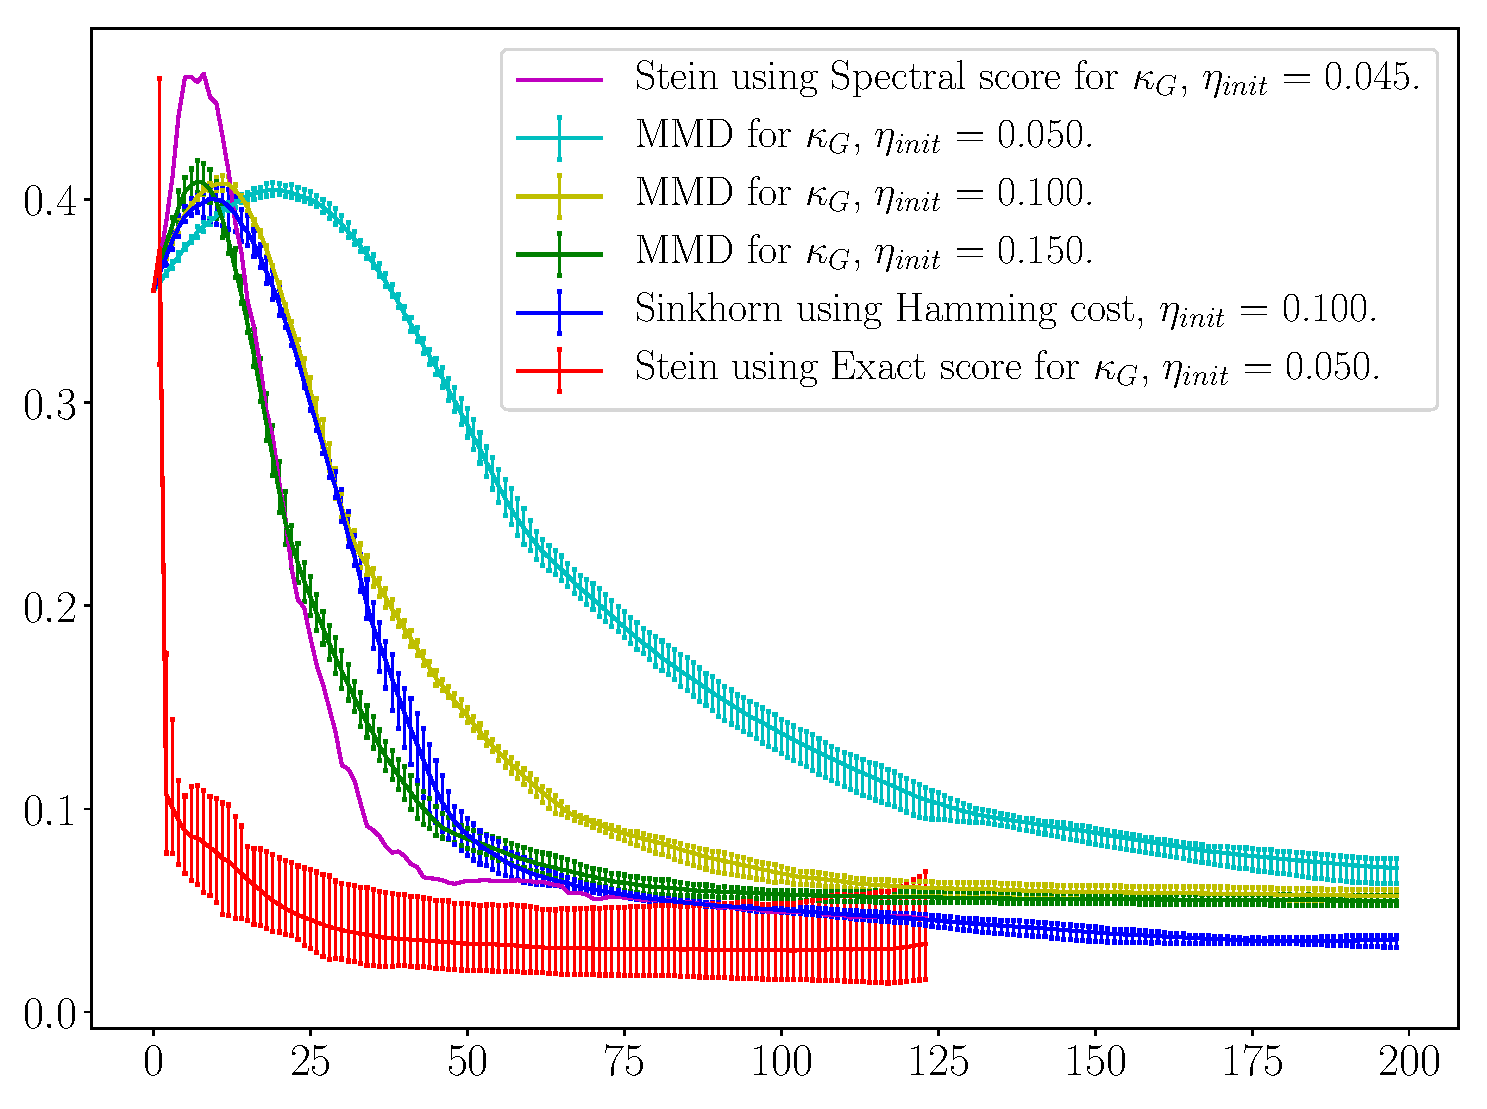
\includegraphics[width=\textwidth, height = 0.8\textwidth]{images/FIG_3a_TV_3_qubits_mmd_stein_sinkhorn_3_evecs_eps_0_08_.pdf}};
  \node[below=of img, node distance=0cm, yshift=1.35cm,font=\color{black}] {epochs};
  \node[left=of img, node distance=0cm, rotate=90, anchor=center,yshift=-0.95cm,font=\color{black}] {$\TV$};
\end{tikzpicture}
        \caption{}
        \label{subfig:tv_3_qubits_mmd_v_sinkhorn}
    \end{subfigure}
    ~ %add desired spacing between images, e. g. ~, \quad, \qquad, \hfill etc. 
      %(or a blank line to force the subfigure onto a new line)
    \begin{subfigure}[t]{0.47\textwidth}
        % \includegraphics[width=\textwidth, height = 0.8\textwidth]{images/Probs_3_qubits_mmd_stein_sinkhorn_3_evecs_eps_0_08_.pdf}
          \begin{tikzpicture}
  \node (img)  {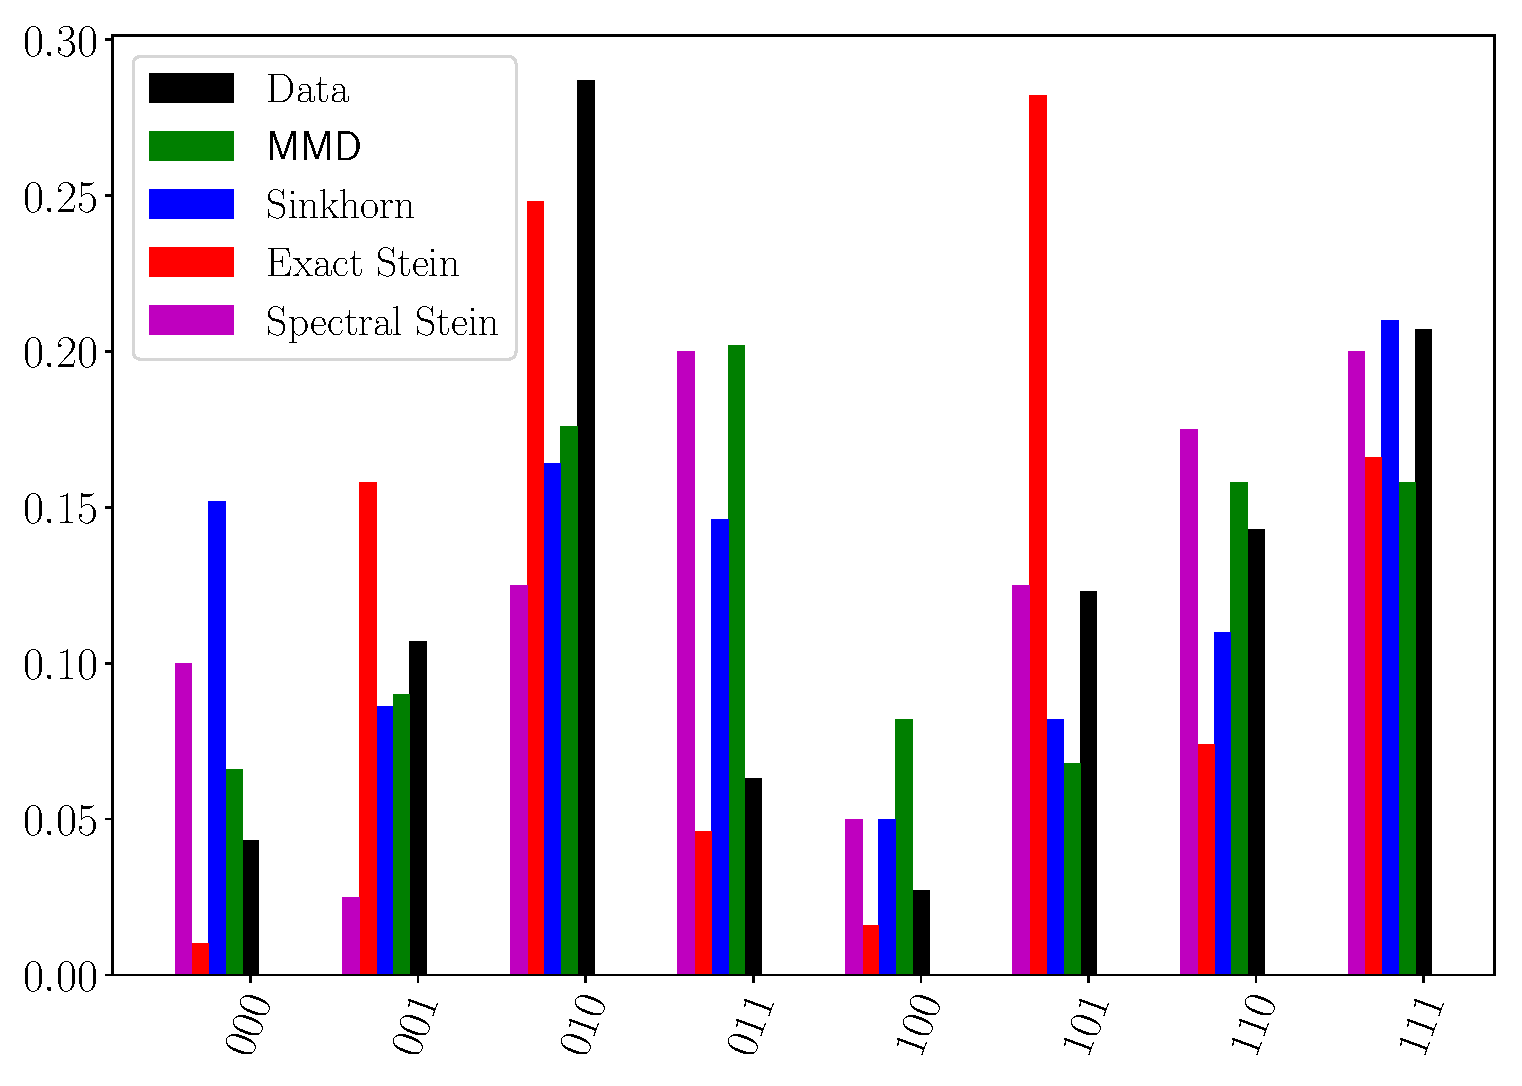
\includegraphics[width=\textwidth, height = 0.8\textwidth]{images/FIG_3b_Probs_3_qubits_mmd_stein_sinkhorn_3_evecs_eps_0_08_.pdf}};
  \node[below=of img, node distance=0cm, yshift=1.35cm,font=\color{black}] {outcomes};
  \node[left=of img, node distance=0cm, rotate=90, anchor=center,yshift=-0.95cm,font=\color{black}] {probability};
\end{tikzpicture}
        \caption{}
        \label{subfig:probs_3_qubits_mmd_mmd_v_sinkhorn}
    \end{subfigure}
\caption{
$\MMD$ [\crule[cyan]{0.2cm}{0.2cm}, \crule[yellow]{0.2cm}{0.2cm}, \crule[ForestGreen]{0.2cm}{0.2cm}] vs.\@ Sinkhorn [\crule[blue]{0.2cm}{0.2cm}] and Stein training with Exact Score function [\crule[red]{0.2cm}{0.2cm}] and Spectral Score method [\crule[magenta]{0.2cm}{0.2cm}] for 3 qubits with fully connected topology, Rigetti {\fontfamily{cmtt}\selectfont 3q-qvm}, \protect\begin{tikzpicture}[transform canvas={scale=0.09}]
%% vertices
\draw[fill=gray] (0,0) circle (20pt);
\draw[fill=gray] (4,0) circle (20pt);
\draw[fill=gray] (2,3) circle (20pt);
%% vertex labels
%%% edges
\draw[gray, thick] (0,0) -- (4,0) -- (0,0) -- (2,3) -- (4,0) -- (2,3);
\end{tikzpicture}
\ \ \ , trained on the data, \eqref{toydatadistribution}. 500 data points are used for training, with 400 used as a training set, and 100 used as a test set. Plots show mean, maximum and minimum values achieved over 5 independent training runs on the same dataset. (a) $\TV$ difference between training methods, with regularisation parameter $\epsilon = 0.08$ for $\SH$, and 3 eigenvectors for Spectral Stein method. Both Sinkhorn divergence and Stein discrepancy are able to achieve a lower $\TV$ than the $\MMD$. (b) Final learned probabilities of each training method. See \appref{supp_matt:numericalresults} for behaviour of corresponding cost functions.
}\label{fig:MMDvSinkvStein3}
\end{figure*}




\begin{figure*}[ht]
    \centering
    \begin{subfigure}[t]{0.23\textwidth}
  \centering
        % \includegraphics[width=\textwidth, height = 0.8\textwidth]{images/TV_4_qubits_ASPEN-4-4Q-A_mmd_sinkhorn_eps_0_1.pdf}
        \begin{tikzpicture}
  \node (img)  {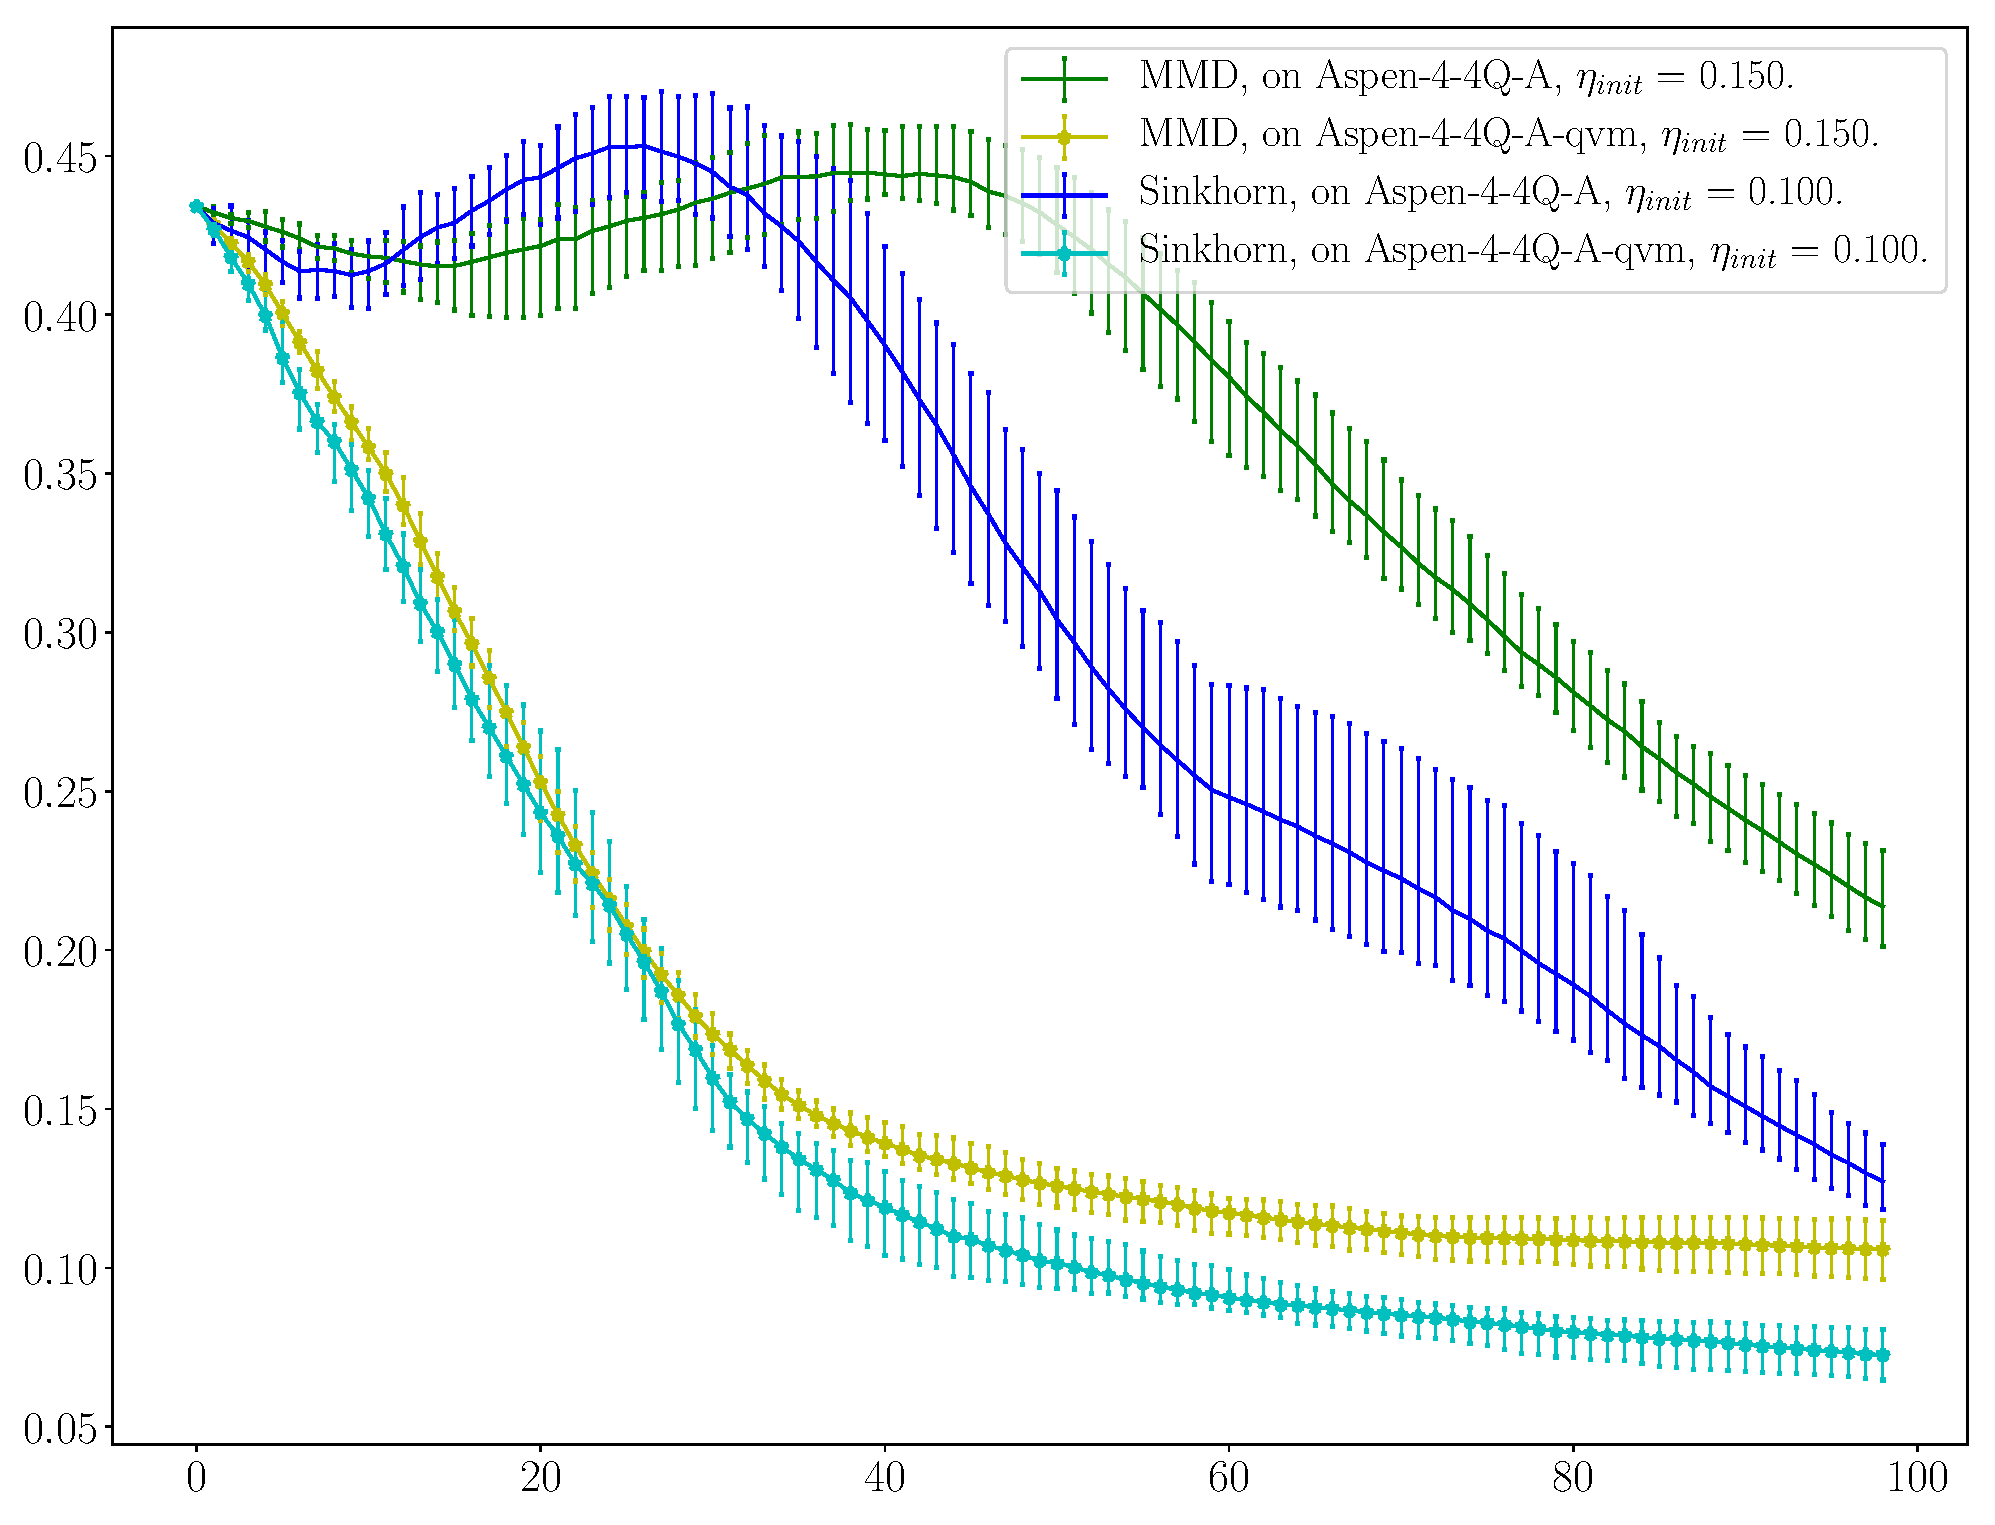
\includegraphics[width=\textwidth, height = 0.8\textwidth]{images/FIG_4a_TV_4_qubits_ASPEN-4-4Q-A_mmd_sinkhorn_eps_0_1.pdf}};
  \node[below=of img, node distance=0cm, yshift=1.35cm,font=\color{black}] {epochs};
  \node[left=of img, node distance=0cm, rotate=90, anchor=center,yshift=-0.95cm,font=\color{black}] {$\TV$};
\end{tikzpicture}
        \caption{}
        \label{subfig:tv_4_qubits_mmd_v_sinkhorn_real}
    \end{subfigure}
    ~
    \begin{subfigure}[t]{0.23\textwidth}
      \centering
        % \includegraphics[width=\textwidth, height = 0.8\textwidth]{images/PROBS_4_qubits_ASPEN-4-4Q-A_mmd_sinkhorn_eps_0_1.pdf}
        \begin{tikzpicture}
  \node (img)  {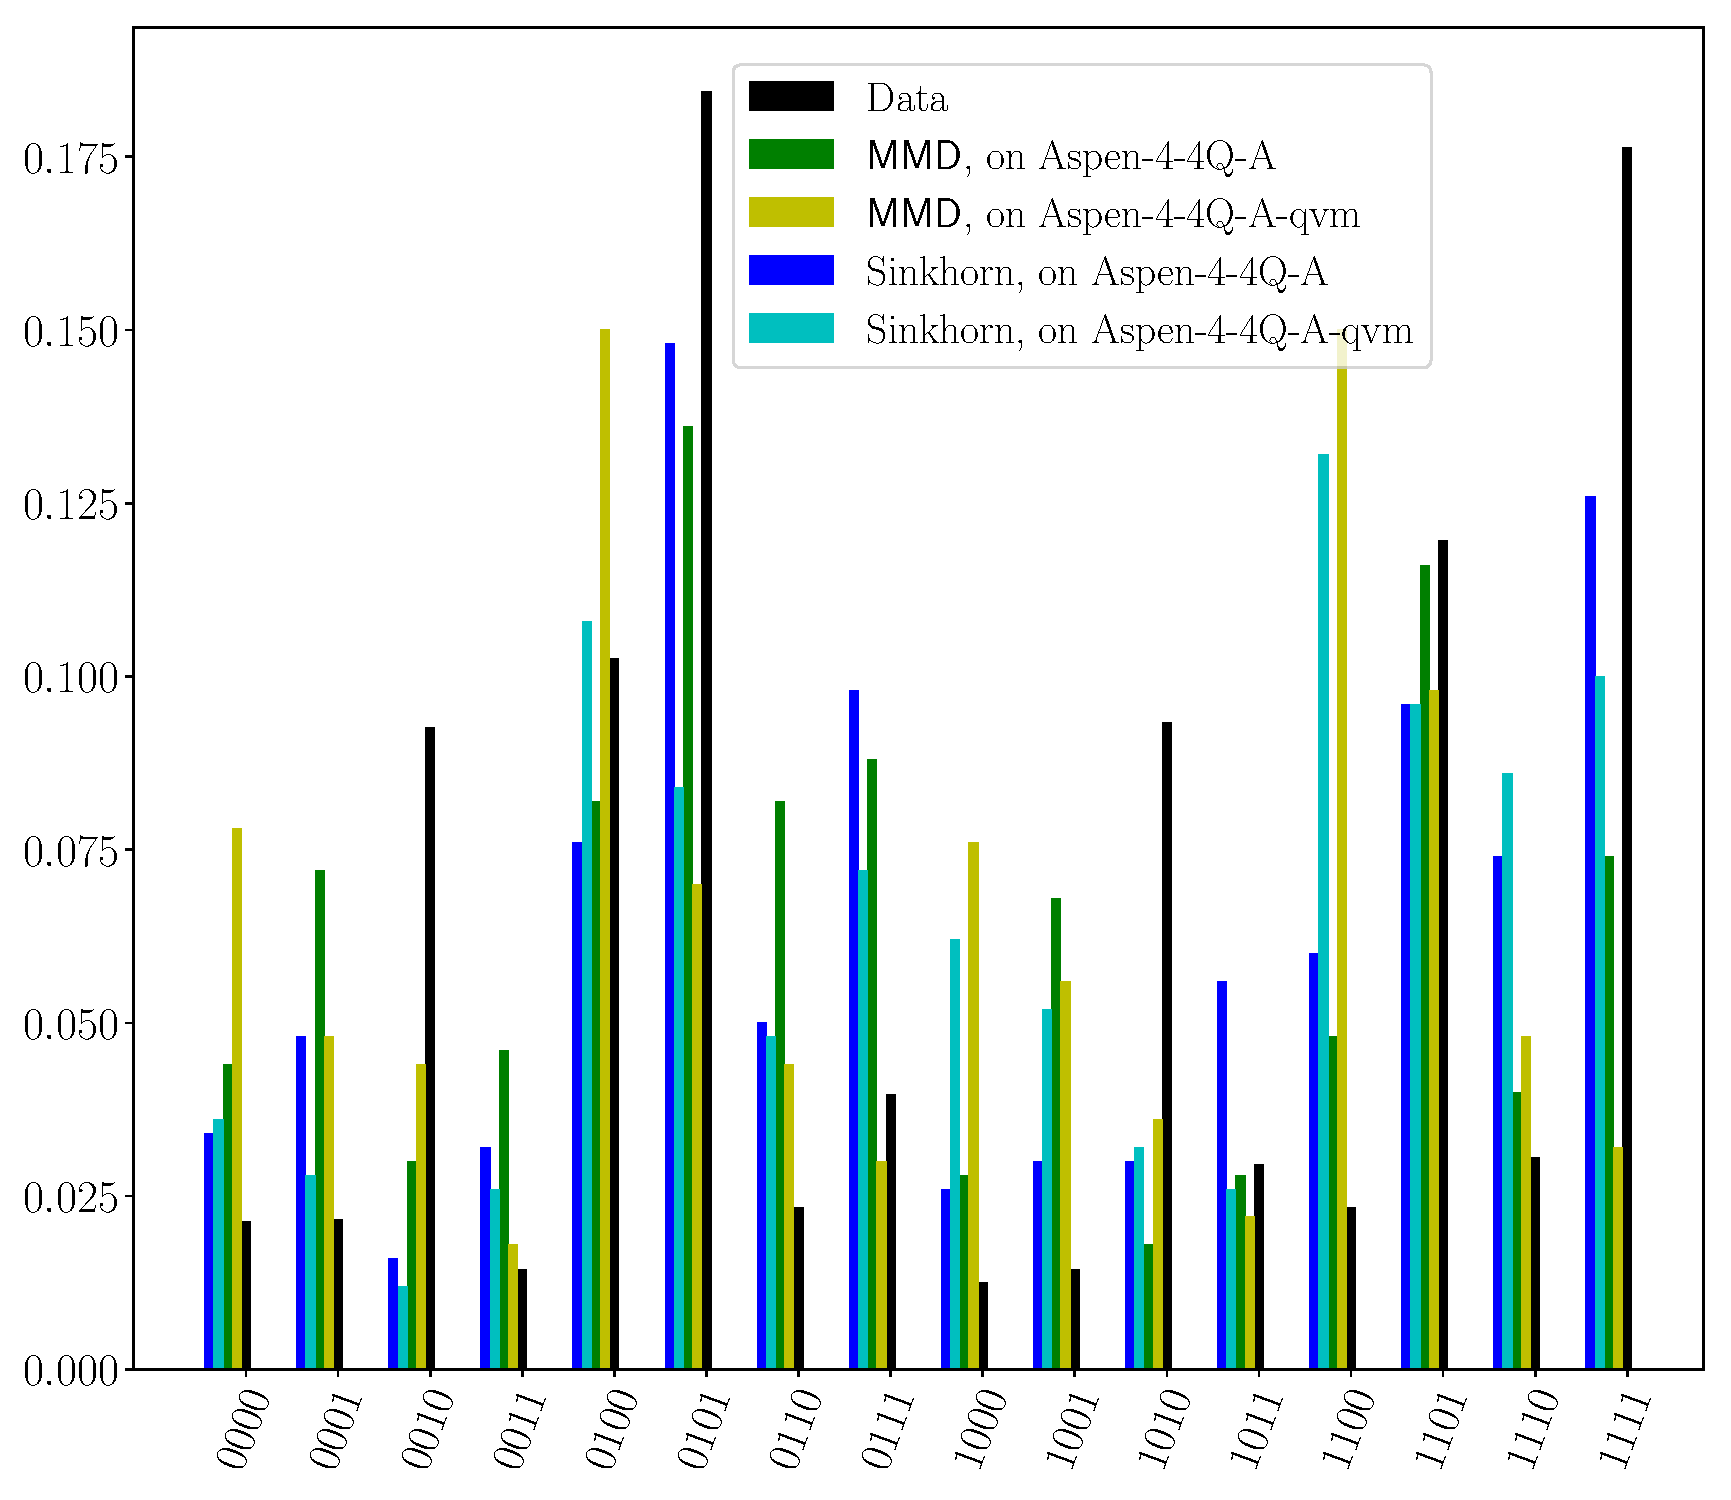
\includegraphics[width=\textwidth, height = 0.8\textwidth]{images/FIG_4b_PROBS_4_qubits_ASPEN-4-4Q-A_mmd_sinkhorn_eps_0_1.pdf}};
  \node[below=of img, node distance=0cm, yshift=1.35cm,font=\color{black}] {outcomes};
  \node[left=of img, node distance=0cm, rotate=90, anchor=center,yshift=-0.95cm,font=\color{black}] {probabilities};
\end{tikzpicture}
        \caption{}
        \label{subfig:probs_4_qubits_mmd_v_sinkhorn_real}
    \end{subfigure}
    ~
    \begin{subfigure}[t]{0.23\textwidth}
      \centering
        % \includegraphics[width=\textwidth, height = 0.8\textwidth]{images/SINK_4_qubits_ASPEN-4-4Q-A_mmd_sinkhorn_eps_0_1.pdf}
        \begin{tikzpicture}
  \node (img)  {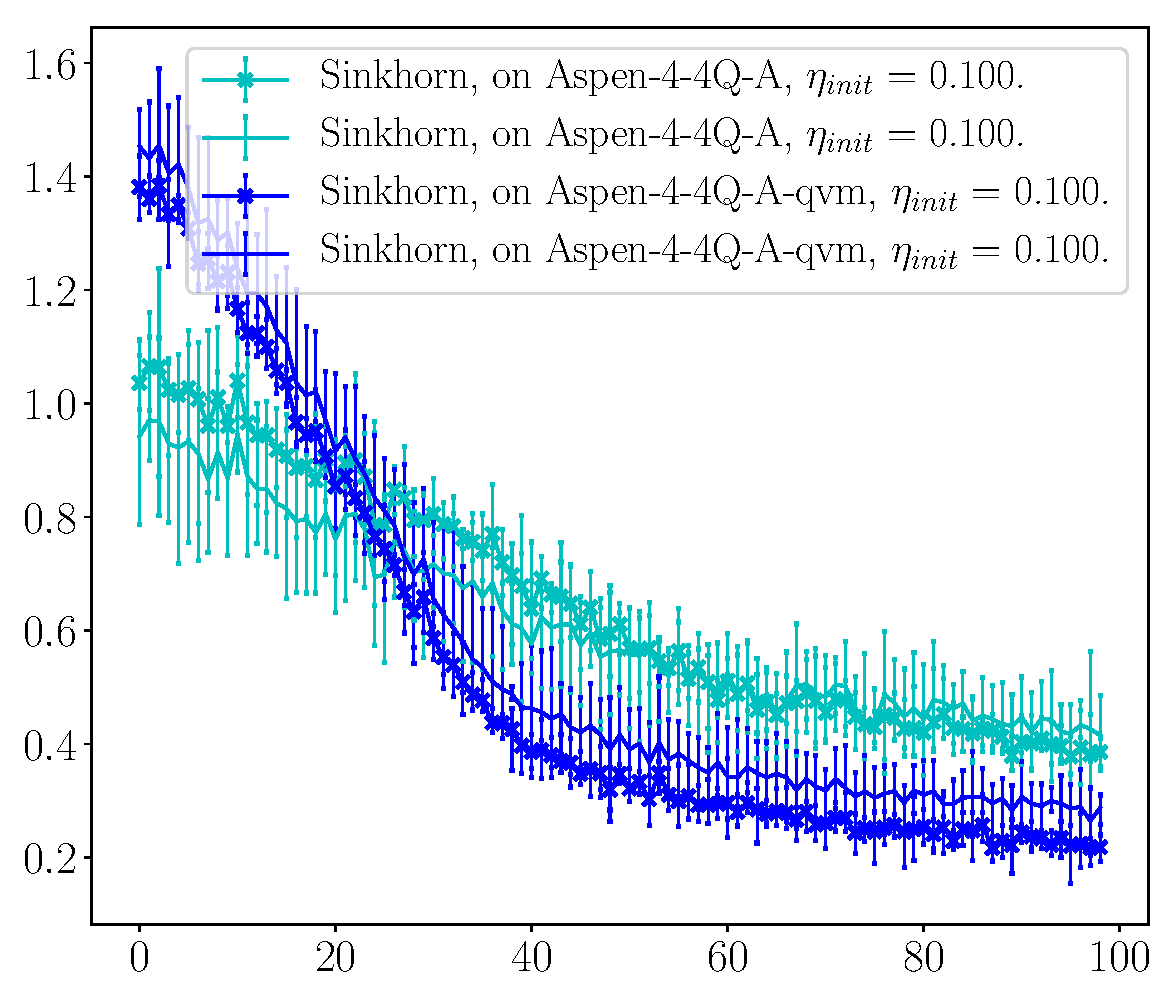
\includegraphics[width=\textwidth, height = 0.8\textwidth]{images/FIG_4c_SINK_4_qubits_ASPEN-4-4Q-A_mmd_sinkhorn_eps_0_1.pdf}};
  \node[below=of img, node distance=0cm, yshift=1.35cm,font=\color{black}] {epochs};
  \node[left=of img, node distance=0cm, rotate=90, anchor=center,yshift=-0.95cm,font=\color{black}] {Sinkhorn loss $\mathcal{L}_{\SH}$};
\end{tikzpicture}
        \caption{}
        \label{subfig:sinkhorn_4_qubits_real}
    \end{subfigure}
    ~
     \begin{subfigure}[t]{0.23\textwidth}
      \centering
        % \includegraphics[width=\textwidth, height = 0.8\textwidth]{images/MMD_4_qubits_ASPEN-4-4Q-A_mmd_sinkhorn_eps_0_1.pdf}
        \begin{tikzpicture}
  \node (img)  {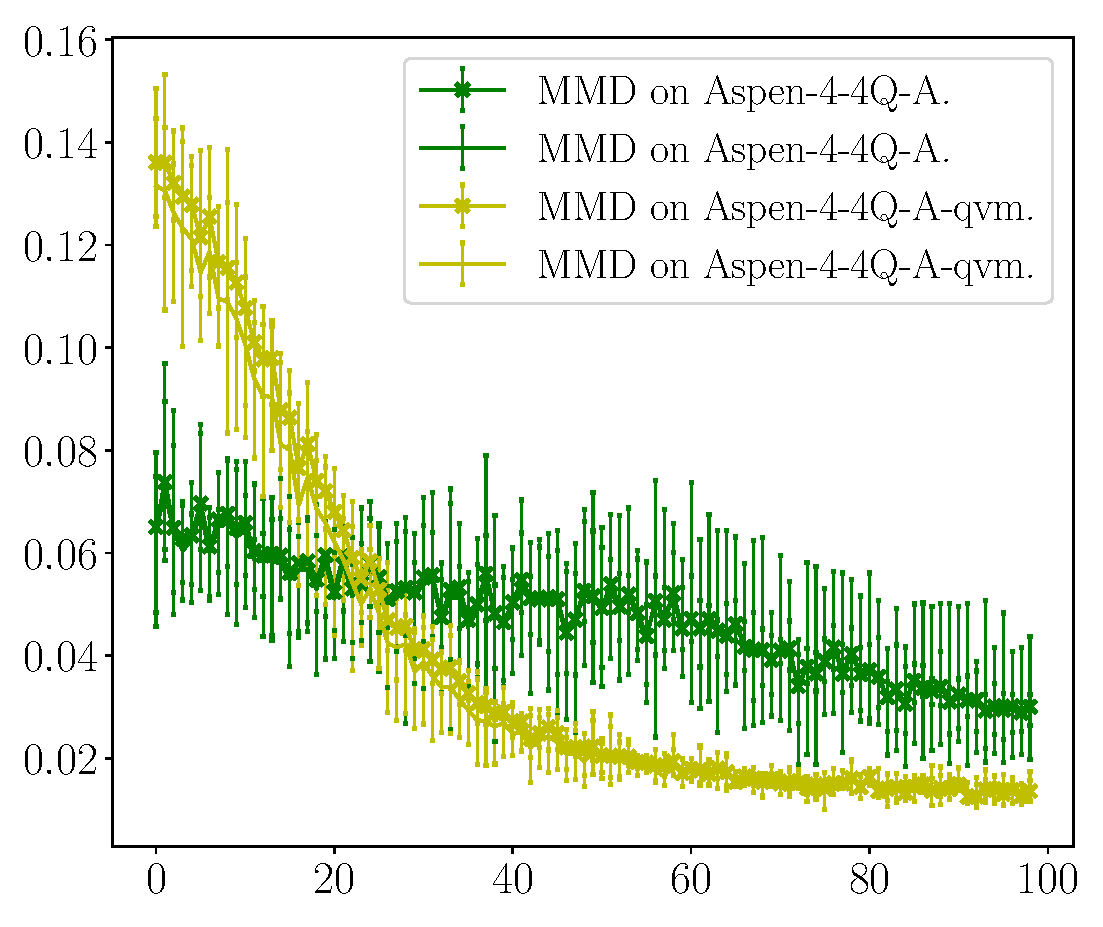
\includegraphics[width=\textwidth, height = 0.8\textwidth]{images/FIG_4d_MMD_4_qubits_ASPEN-4-4Q-A_mmd_sinkhorn_eps_0_1.pdf}};
  \node[below=of img, node distance=0cm, yshift=1.35cm,font=\color{black}] {epochs};
  \node[left=of img, node distance=0cm, rotate=90, anchor=center,yshift=-0.95cm,font=\color{black}] {$\MMD$ loss $\mathcal{L}_{\MMD}$};
\end{tikzpicture}
        \caption{}
        \label{subfig:mmd_4_qubits_real}
    \end{subfigure}
    ~
    %   \begin{subfigure}[t]{0.24\textwidth}
    %  \centering
    %     \includegraphics[width=0.9\textwidth]{images/4qubit_Aspen_4_4Q_A.pdf}
    %     \vskip 5pt
    %     \caption{Qubit `line' topology in Rigetti {\fontfamily{cmtt}\selectfont Aspen-4-4Q-A} chip, using qubits, $(0, 1, 2, 7)$.}
    %     \label{subfig:4_qubit_topology_aspen_4_4q_a}
    % \end{subfigure}
    \caption{$\MMD$ [\crule[ForestGreen]{0.2cm}{0.2cm}] vs.\@ Sinkhorn [\crule[blue]{0.2cm}{0.2cm}] for 4 qubits comparing performance on the real QPU ({\fontfamily{cmtt}\selectfont Aspen-4-4Q-A}) vs.\@ simulated behaviour on QVM ({\fontfamily{cmtt}\selectfont Aspen-4-4Q-A-qvm}) using 500 samples and a batch size of 250, learning target data [\crule[black]{0.2cm}{0.2cm}]. (a)$\TV$ Difference between training methods with regularisation parameter $\epsilon = 0.1$ (b) Final learned probabilities, (c) $\mathcal{L}^{0.1}_{\SH}$ on QVM  [\crule[blue]{0.2cm}{0.2cm}] vs.\@ QPU  [\crule[cyan]{0.2cm}{0.2cm}]. (d) $\mathcal{L}_{\MMD}$ on QVM  [\crule[ForestGreen]{0.2cm}{0.2cm}] vs.\@ QPU  [\crule[cyan]{0.2cm}{0.2cm}]. }\label{fig:MMDvSink4_real}
\end{figure*}


\subsection*{Hardness and Quantum Advantage}
It is crucially important, not just for our purposes, but for the design of quantum machine learning algorithms in general, that the algorithm itself is providing some advantage over \textit{any} classical one, for the same task. This is the case for so-called \textit{coherent} algorithms, like the HHL linear equation solver\cite{harrow_quantum_2009}, which is $\BQP$-complete, and therefore unlikely to be fully dequantised, 
%by a classical algorithm achieving a similar runtime. 
However, such a proven advantage for \textit{near term} QML algorithms is yet out of reach. We attempt to address such a question in two steps. 
\begin{enumerate}
    \item We show that for a large number of parameter values, $\boldsymbol\theta$, our $\IBM$ circuits are `hard', that is to say cannot be efficiently simulated classically up to a multiplicative error, in the worst case. We also show that this holds for the quantum circuits generated via the gradient computation, and hence the model may \textit{remain} hard during training (although we do not know for sure).
    \item We provide the first formal definitions for quantum learning supremacy, the ability of a quantum model to provably outperform all classical models in a certain task, and a potential pathway to prove such a thing.
\end{enumerate}

The \emph{intuition} behind the second point is the following. If our $\IBM$ model could %for instance, 
learn a target distribution $\pi$ in the sense of providing a quantum circuit $C$
close to $\pi$ up to a given error in total variation,
and $C$ had %is believed to itself 
quantum supremacy, then the model would have demonstrated something which is likely classically unfeasible. Otherwise, it would mean that there exists a efficient classical algorithm 
which can get close to $\pi$ without repeatedly sampling and simulating quantum circuits 
en route.

The first point does not completely fit that intuition. For one thing, it is not known to hold itself to within the required notion of error (i.e.\@ total variation distance). Also, even though the model is more \textit{expressive} than any classical model\cite{du_expressive_2018}, this does not imply that it could actually \textit{learn} a hard distribution. On the other hand, it is easy to see why the converse would be true, if the $\IBM$ could learn a model which is hard to sample from classically, the underlying circuit must have, at some point, reached a circuit configuration for which the output distribution is hard to classically sample.

We can address point 1. informally (see \appref{supp_matt:hardness} for the formal statements and proof) in three steps:
\begin{itemize}
    \item If the initial parameters of the model $\{\boldsymbol \alpha\} = \{J_{ij}, b_k\}\in\{0,\frac{\pi}{8}, \dots, \frac{7\pi}{8}\}$ and final measurement angles are chosen such that $U_f \left( \mathbf{\Gamma}, \mathbf{\Delta}, \mathbf{\Sigma} \right) = H^{\otimes n}$, then the resulting $\IBM$ circuit class will be hard to simulate up to an additive error of $1/384$ in total variation distance, subject to a conjecture relating to the hardness of computing the Ising partition function \cite{bremner_average-case_2016}.
    \item If certain configurations of the parameters are chosen to be either of the form, $(2l+1)\pi/kd$, where $l, d$ are integers, and $k$ is a number which depends on the circuit family, or in the form $2\pi\nu$, where $\nu$ is irrational, then the resulting class of circuits will be hard to sample from classically, up to a multiplicative error, in the worst case.
    \item The circuits produced at each epoch as a result of the gradient updates will each result in a hard circuit class as long as the gradient updates are not chosen carelessly. In each epoch, if the update step is constrained in a way that the new value of the parameter 
$\theta^{d+1}_k= \theta_k^{d} - \eta\partial_{\theta_k}\mathcal{L}_B$ does not become rational, then the updated circuits will also belong to a class which is hard to simulate. This is because the updates can simply be absorbed into the original gates, to give a circuit which has the same form. This holds also for the gradient shifted circuits in\eqref{circuit:gradientplusminuscircuit} since these correspond to circuits whose parameters are updated as follows: $\theta^{d, \pm}_k \leftarrow \theta_k^{d} \pm \pi/2$.
\end{itemize}

We now provide definitions informally to match the requirements of the second point. We adapt definitions from distribution learning theory\cite{kearns_learnability_1994} for this purpose. Specifically, we say that a generative QML Algorithm, $\mathcal{A}\in \BQP$ (with a small abuse of notation) has %demonstrated 
\textit{quantum learning supremacy} (QLS) if there exists a class of probability distributions 
$\mathcal{D}_n$ over $\mathcal X^n$ (bit vectors of length $n$), 
for which there exists a metric $d$, and a fixed $\epsilon$ such that 
$\mathcal{D}_n$ is $(d ,\epsilon, \BQP)$-learnable via $\mathcal{A}$, 
but not $\left( d ,\epsilon, \BPP \right)$-learnable (i.e.\@ learnable by a purely classical algorithm). The task of the learning algorithm $\mathcal{A}$ is, given a target distribution $D\in \mathcal D_n$,
to output, with high probability, a \textit{Generator}, 
$\GEN_{D'}$, for a distribution $D'$, 
such that $D'$ is close to $D \in \mathcal{D}_n$ with respect to the metric $d$. 
For the precise definitions of learnability we employ see \appref{supp_mat:superioritydefinitions}.
This framework is very similar to that of, and inspired by, probably approximately correct (PAC) learning, which has been well studied in the quantum case\cite{arunachalam_survey_2017}, but applies more closely to the task of supervised learning. It is known that in certain cases, the use of quantum computers can be beneficial to PAC learning, but not generically\cite{arunachalam_quantum_2019}. Based on this, it is possible that there exist some classes of distributions which cannot be efficiently learned by classical computers ($\BPP$ algorithms), but which could be learned by quantum devices ($\BQP$ algorithms). The motivation for this is exactly rooted in the question of quantum supremacy, and illustrated crudely in \figref{subfig:qlsillustration}. 

An initial attempt at QLS is as follows. As mentioned above, if random $\IQP$ circuits could be classically simulated to within a $\TV$ error of $\epsilon = 1/384$\cite{bremner_average-case_2016} in the worst case (with high probability over the choice of circuit), this would imply unlikely consequences for complexity theory. Now, if a generative quantum model was able to achieve a closeness in $\TV$ less than this constant value, perhaps by minimising one of the upper bounds in \eqref{tv_wasserstein_sinkhorn_inequality}, then we could claim this model had achieved something classically intractable, and could not be classically simulated either. For example if we make the following assumptions,
\begin{enumerate}
    \item Assume the $\IBM$ could achieve a $\TV < \delta$ to a target $\IQP$ distribution. 
    \item Assume a classical probabilistic algorithm, $\mathcal{C}$, could output a distribution $q$ in polynomial time which was $\gamma$ close in $\TV$ to the $\IBM$, i.e.\@ it could simulate it efficiently.
\end{enumerate}
Then:
\begin{align}
&\TV(p_{\IQP}, q) = \frac{1}{2}\sum_{\mathbf{x}}|p_{\IQP}(\mathbf{x})-q(\mathbf{x})| \nonumber\\
&= \frac{1}{2}\sum_{\mathbf{x}}|p_{\IQP}(\mathbf{x}) - p_{\boldsymbol\theta}(\mathbf{x}) + p_{\boldsymbol\theta}(\mathbf{x})-q(\mathbf{x})|\nonumber\\
&\leq \frac{1}{2}\sum_{\mathbf{x}}|p_{\IQP}(\mathbf{x}) -p_{\boldsymbol\theta}(\mathbf{x})| +\frac{1}{2}\sum_{\mathbf{x}}|p_{\boldsymbol\theta}(\mathbf{x})-q(\mathbf{x})|\nonumber\\
&\leq \delta+\gamma \equiv \epsilon
\end{align}

\noindent where the third line follows from the triangle inequality. Therefore $\mathcal{C}$ could simulate an $\IQP$ distribution also, and we arrive at a contradiction. The major open question left by this work is whether QLS is possible at all; can a quantum model outperform all classical ones in generative learning?


\begin{figure*}[ht]
\centering
%
\begin{subfigure}[t]{0.5\textwidth}
%    \centering
    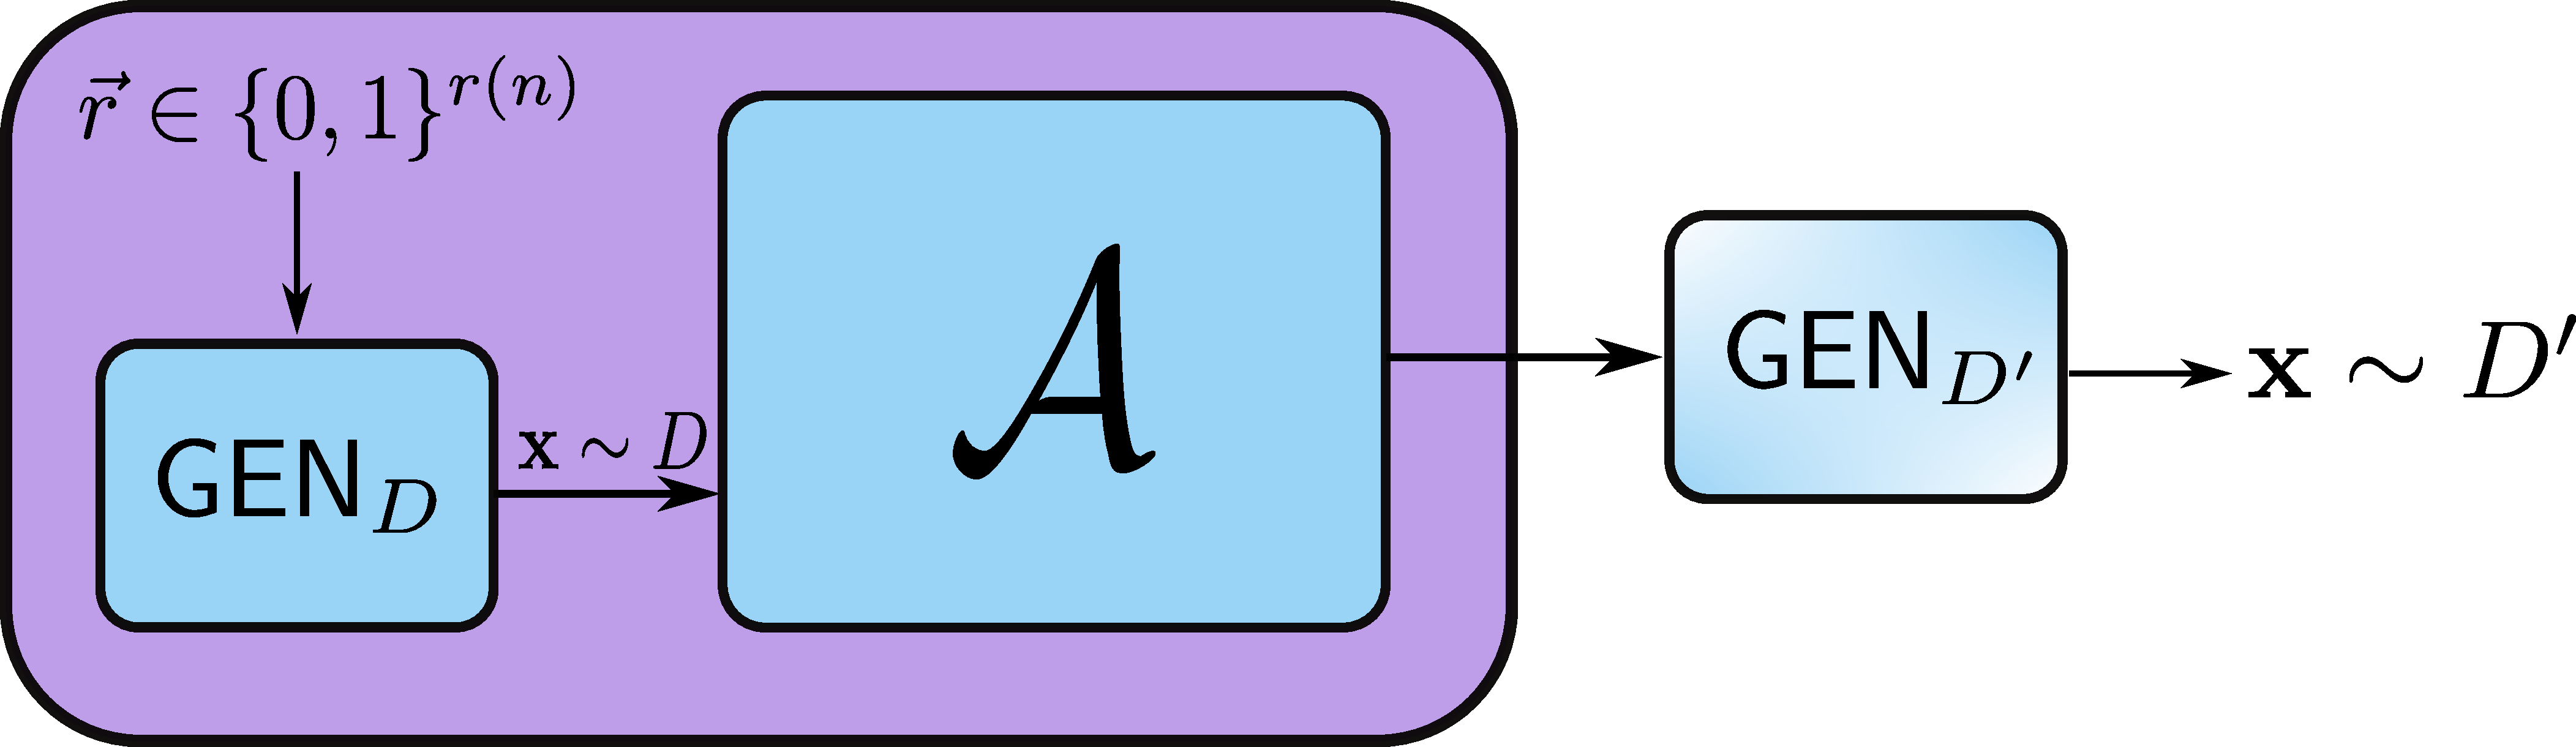
\includegraphics[width=\textwidth, height = 0.3\textwidth]{images/FIG_5a_generator.pdf}
    \caption{}\label{subfig:generator}
\end{subfigure}
%
\qquad
\begin{subfigure}[t]{0.4\textwidth}
%\centering
        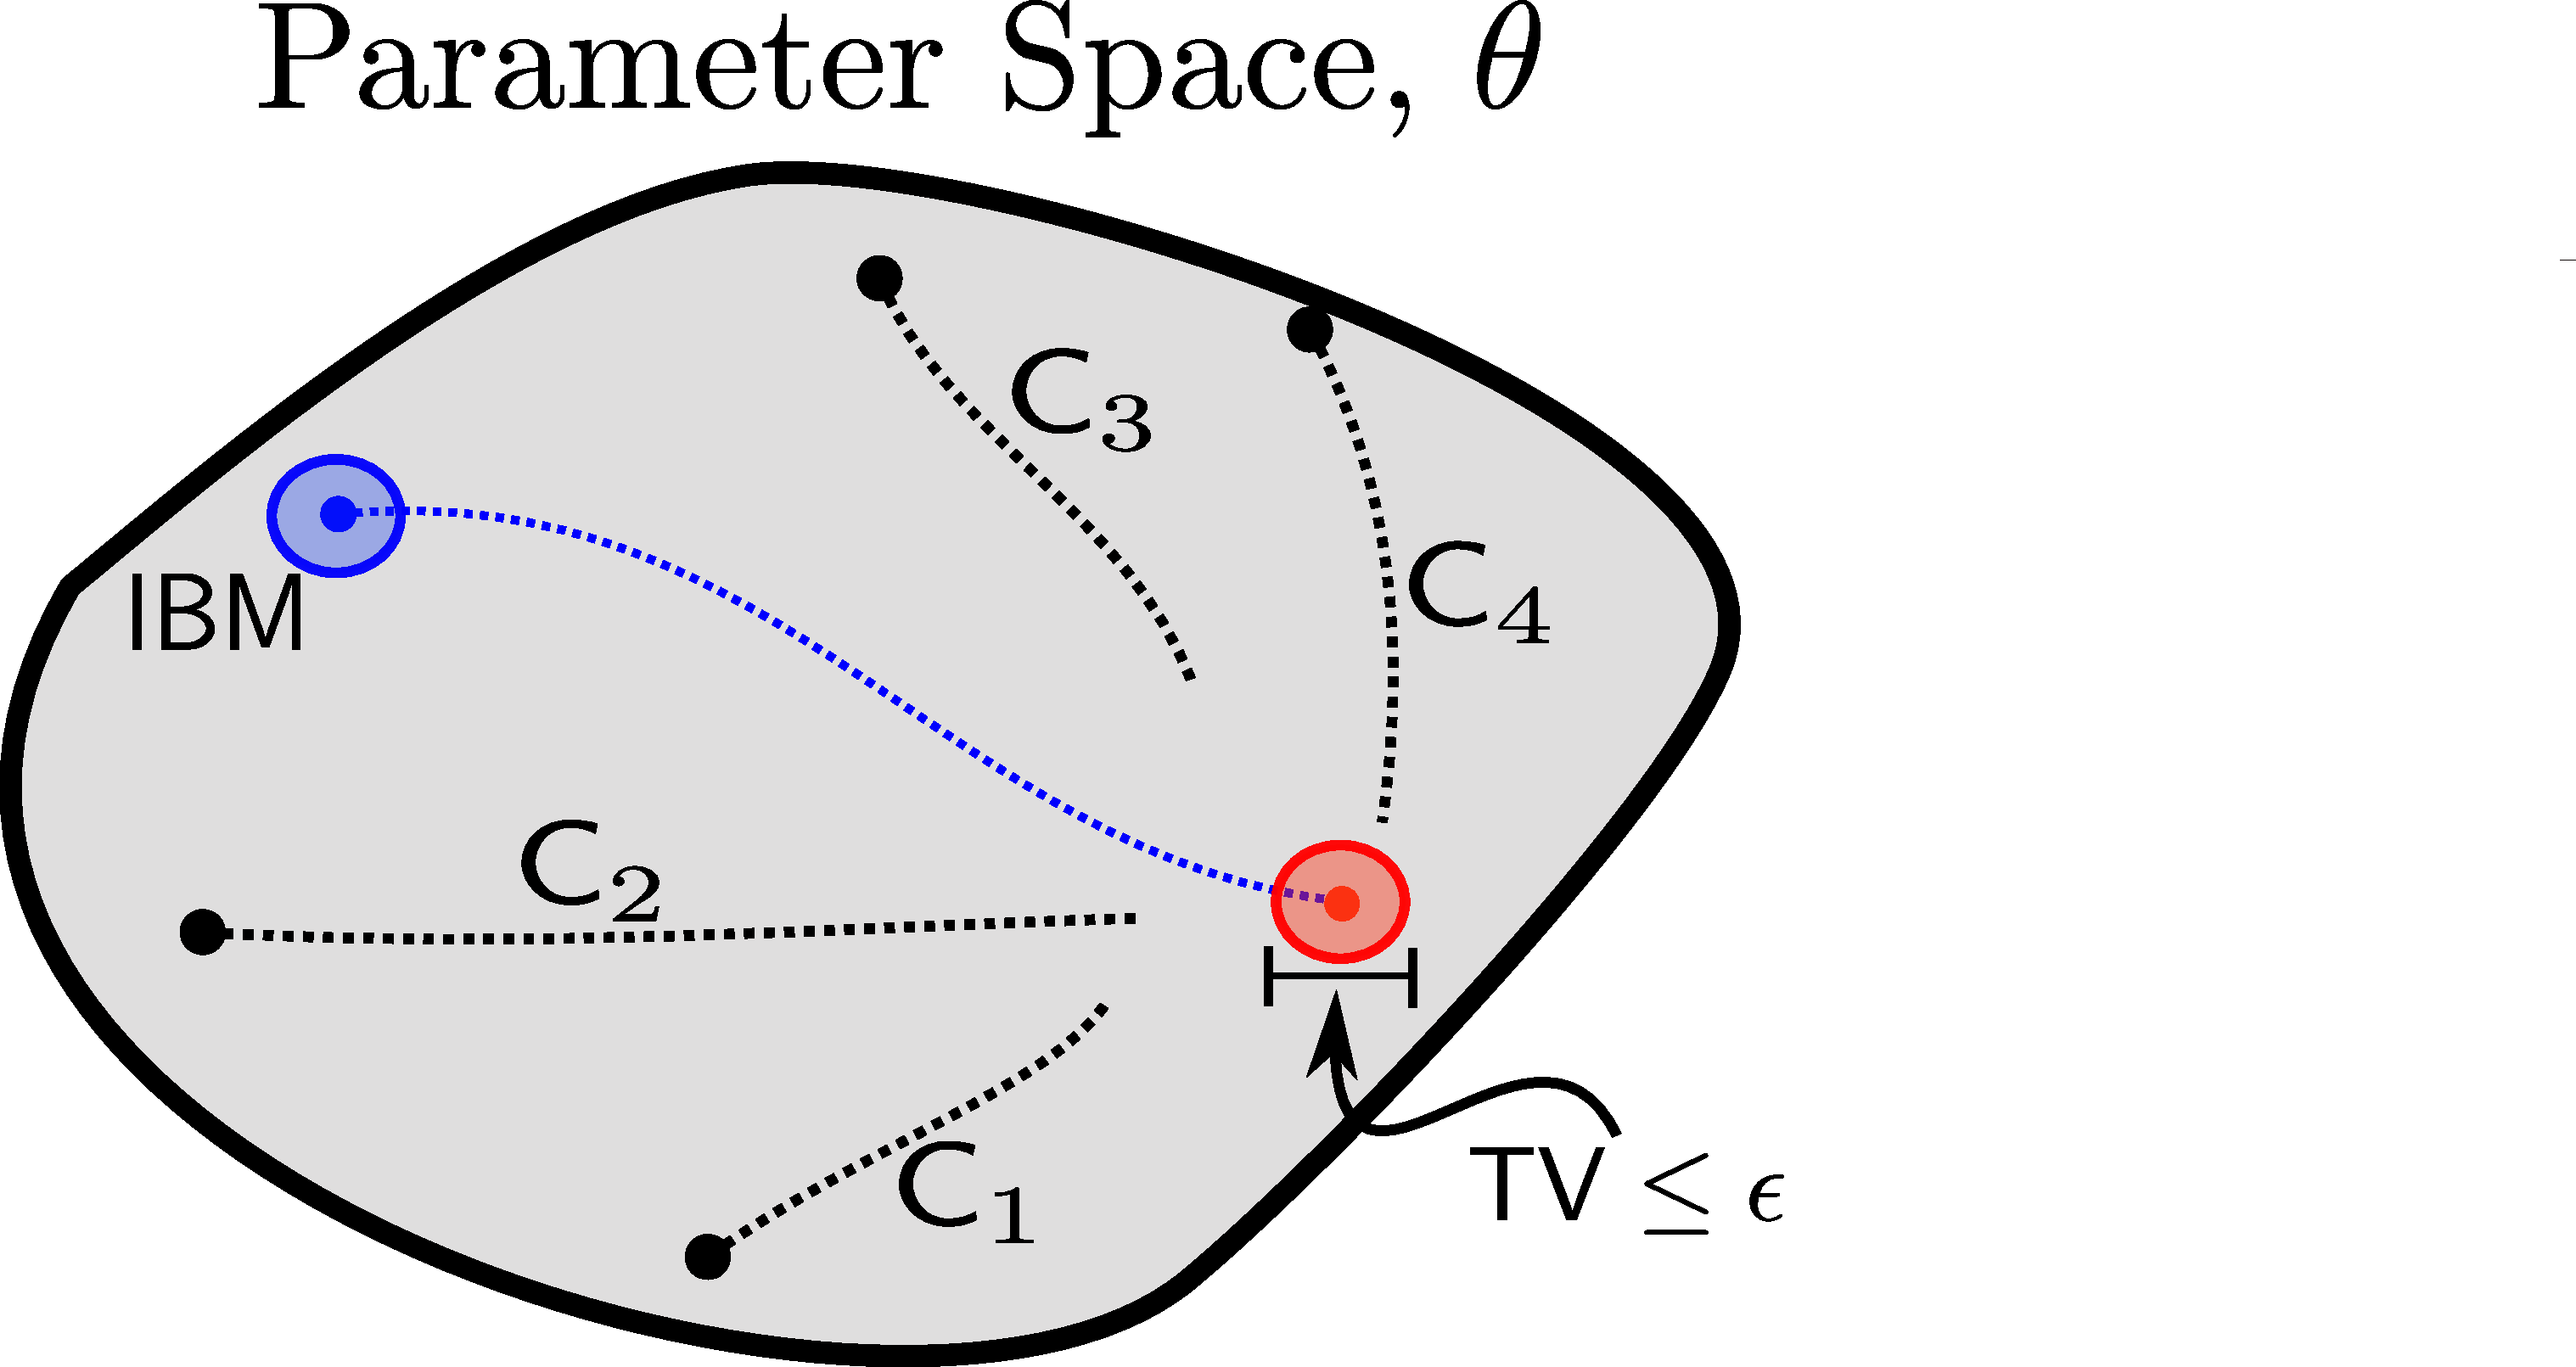
\includegraphics[width=\textwidth, height = 0.5\textwidth]{images/FIG_5b_tv_hardness_parameter_space.pdf}
    \caption{}
    \label{subfig:qlsillustration}
\end{subfigure}
\caption{
%(a) Hybrid training procedure of Ising Born Machine. 
(a) Illustration of a learning procedure using a Generator. The algorithm 
$\mathcal A$ is given access to $\GEN_D$, which provides samples, $\mathbf{x}\sim D$, and must output a Generator for a distribution which is close to the original. We allow the target generator to be classical, hence it may take as input a string of random bits, of size polynomial in $n$, $r(n)$, if not able to generate its own randomness. (b) Crude illustration of quantum learning supremacy. No classical algorithm, $\mathcal{C}_i$, should be able to achieve the required closeness in total variation to the target distribution, but the $\IBM$ (or similar) should be able to, for \textit{some} class of target distributions. There should be some path in the parameter space of the $\IBM$, $\boldsymbol\theta$, which achieves this.
}\label{fig:learning_supremacy}
\end{figure*}


\subsection*{Quantum Compiling}
As a concrete application of such a model outside the scope of classical generative modelling, we can use the $\IBM$ training to perform a type of `weak' quantum circuit compilation. To the best of our knowledge, this is a novel instance of applying techniques in generative modelling to quantum information processing tasks. There are also potentially other areas which could be studied using these tools, but this is beyond the scope of this work.

The major objective in this area is to compile a given target unitary, $U$, into one which consists exclusively of operations available to the native hardware of the Quantum Computer in question. For example, in the case of Rigetti's Aspen QPU, the native gates are the following set: $\{R_x(\pm \pi/2), R_z(\theta), CZ\}$ \cite{smith_practical_2016, khatri_quantum-assisted_2018}, and any unitary which a user wishes to implement must be compiled into a unitary $V$ which contains only these ingredients. Potential solutions to this problem\cite{jones_quantum_2018, khatri_quantum-assisted_2018} involve approximating the target unitary, $U$ itself by assuming $V$ is a parametric circuit built from the native gates which can be trained by some optimisation strategy. We adopt a similar view here, but we do not require any extra quantum resources to perform the compilation. With this limitation, we make a tradeoff in that we are not guaranteed to apply \textit{the same} target unitary, only that the output distribution will be somewhat close to that produced by the target. Clearly this is a much weaker constraint than the task of compiling directly one unitary into another, since many unitaries may give rise to the same distribution but it is much closer to the capabilities of near term devices. To illustrate this application, we train an $\IBM$ to learn the output distribution of a random $\IQP$ circuit when restricted to a $\QAOA$ architecture itself using $\mathcal{L}_{\SH}$ as a cost function.
\begin{multline}
    \IBM\left(\left\{J^{\QAOA}_{ij}, b^{\QAOA}_k\right\}, \left\{\Gamma_k = \frac{\pi}{4}\right\}, 0,  0\right) \\
    \overset{Compile}{\rightarrow}   \IBM\left(\left\{J^{\IQP}_{ij}, b^{\IQP}_k\right\}, \left\{\Gamma_k = \frac{\pi}{2\sqrt{2}}\right\}, \right.\\0, \left.\left\{\Sigma_k = \frac{\pi}{2\sqrt{2}}\right\}\right)
\end{multline}

\noindent The measurement unitary at the end of the circuit makes this process non-trivial, since this will give rise to significantly different distributions, even given the same parameters in $U_z$. We illustrate this in \figref{fig:autocompilationtwoqubits} using the Rigetti {\fontfamily{cmtt}\selectfont 2q-qvm} and for three qubits in \appref{supp_matt:numericalresults}. We find that even though the learned parameter values are different from the target, the resulting distributions are quite similar, as expected.

\begin{figure*}[ht]
\centering
\begin{subfigure}[t]{0.12\textwidth}
    \centering
    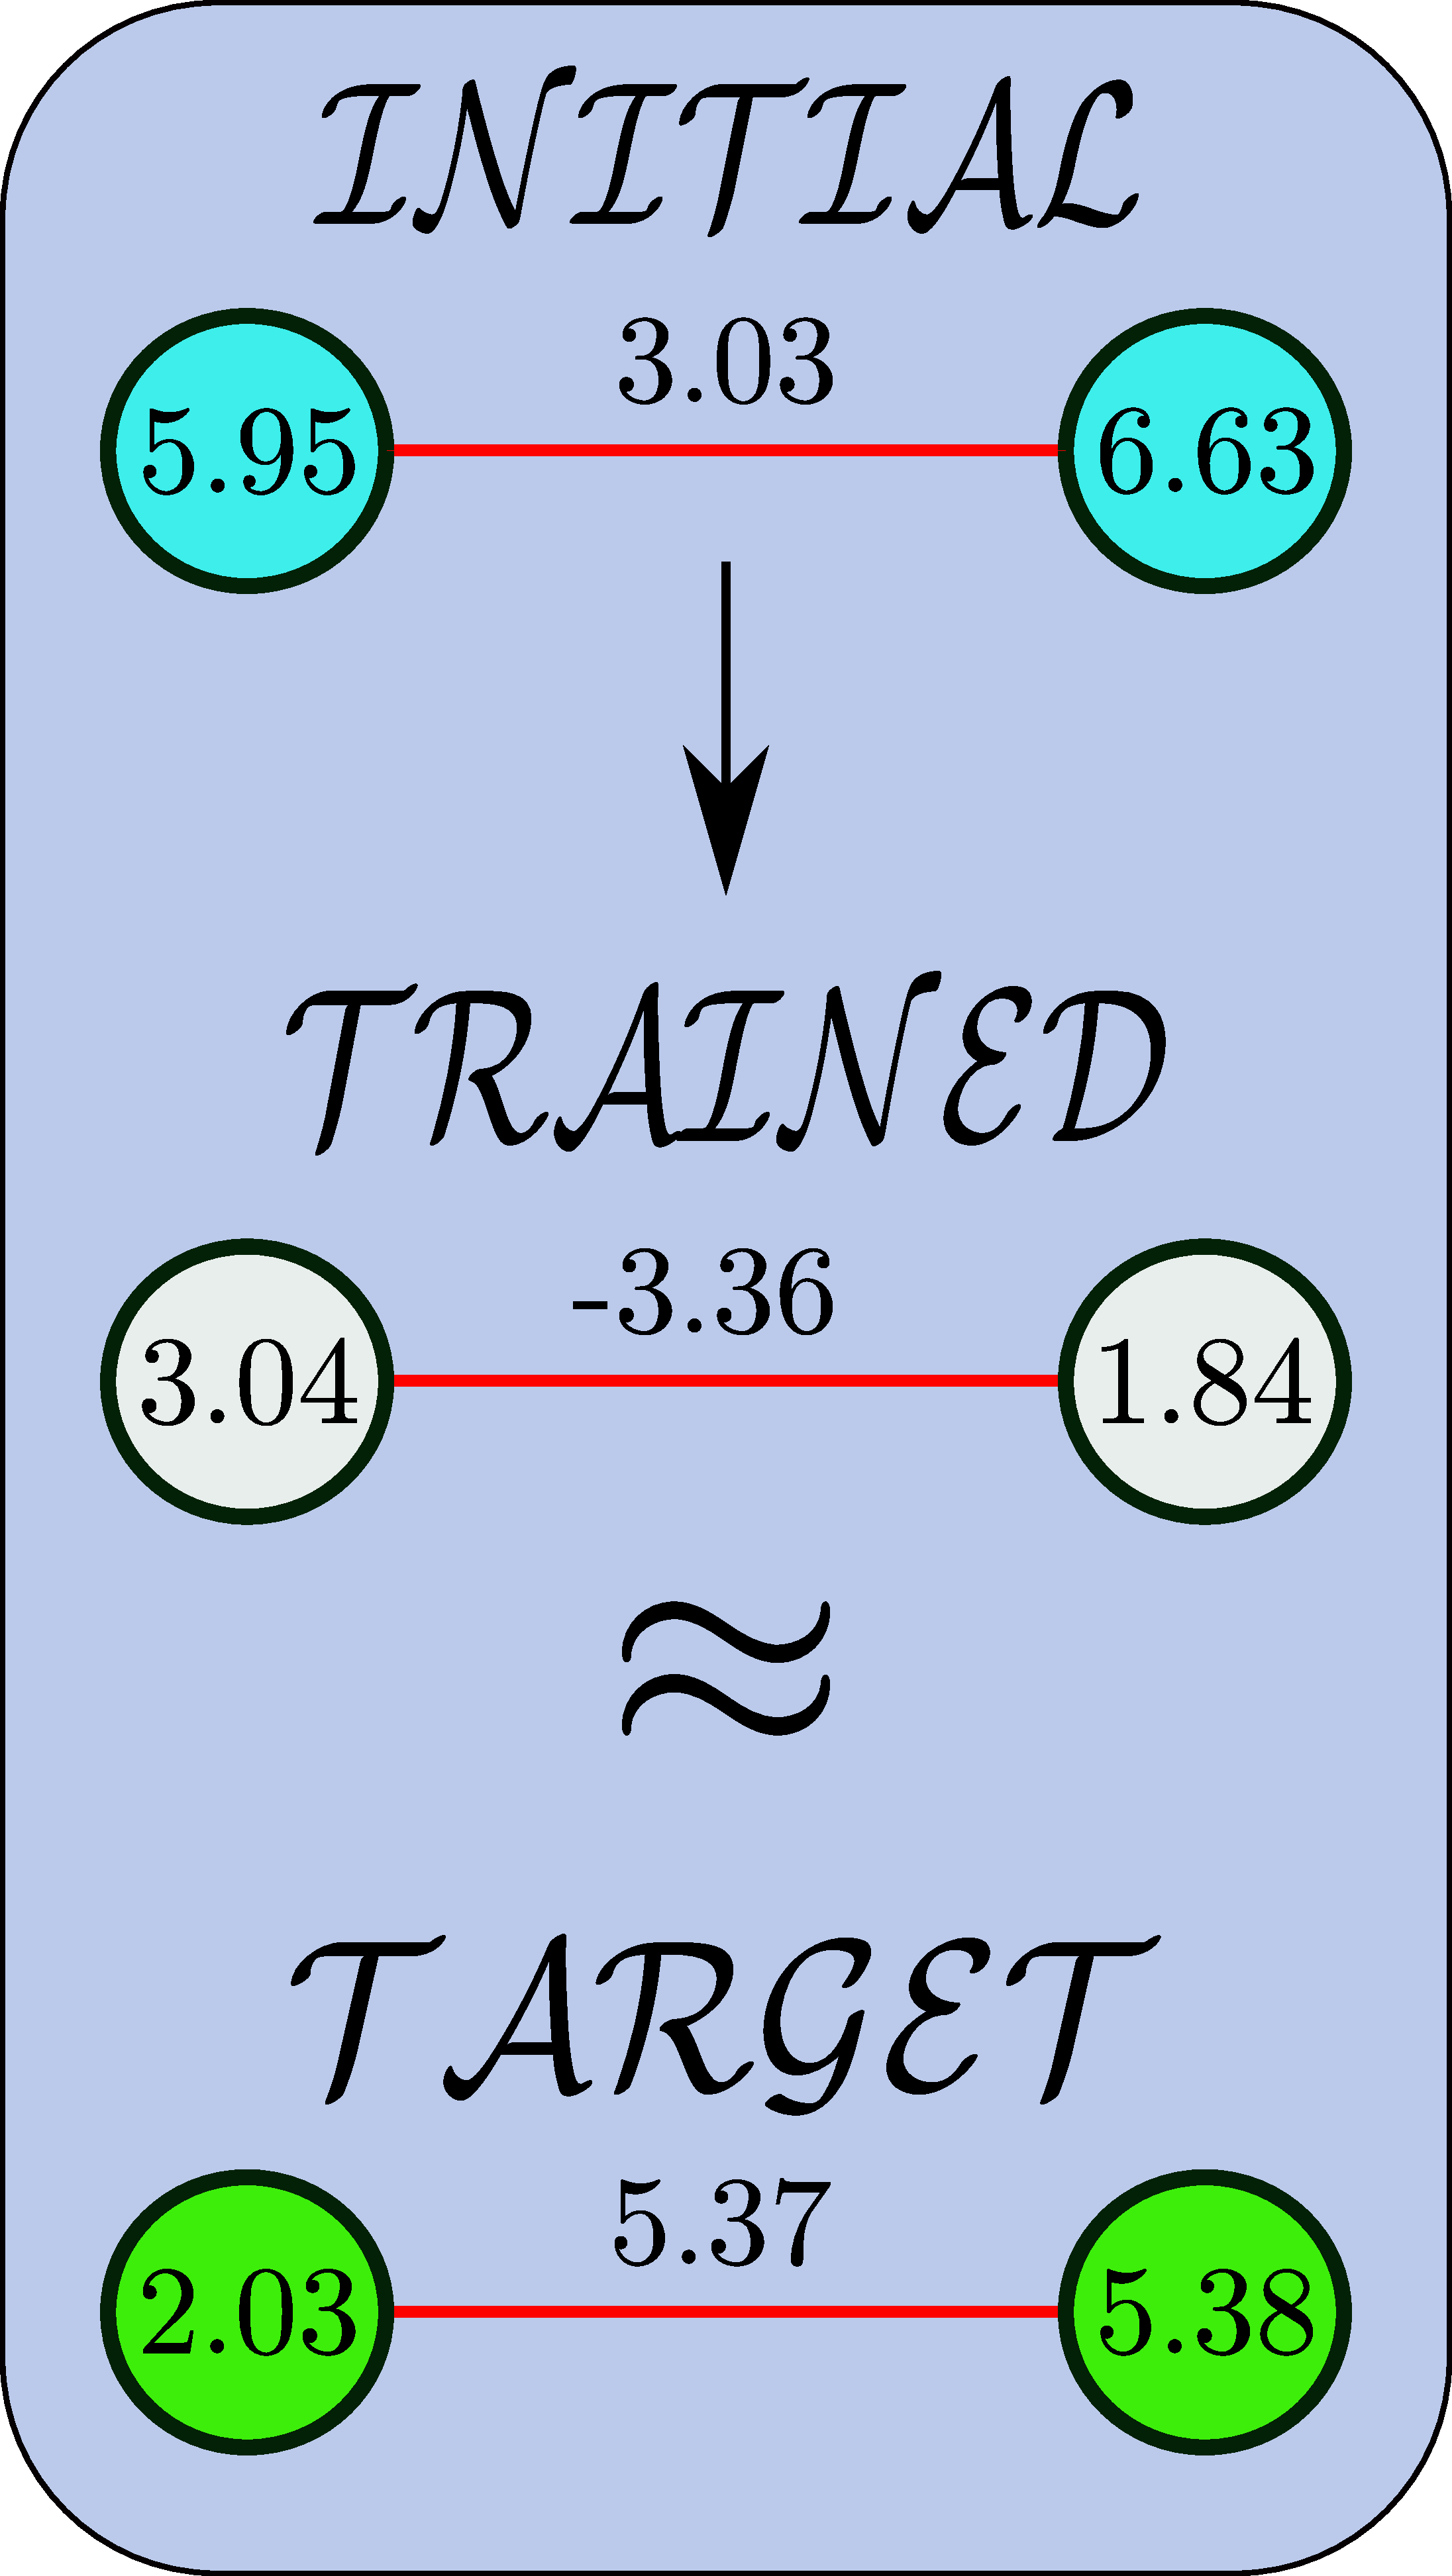
\includegraphics[width=\textwidth, height = 1.8\textwidth]{images/FIG_6a_circuit_init_two_qubits_vertical.pdf}
    \caption{}\label{subfig:auto_comp_2_params}
\end{subfigure}
~
\begin{subfigure}[t]{0.27\textwidth}
        \centering
        % \includegraphics[width=\textwidth, height = 0.8\textwidth]{images/compilation_probs_2_qubits_qaoa_to_IQP_sinkhorn_eps_0_1_lr_0_05_AVERAGE.pdf}
     \begin{tikzpicture}
  \node (img)  {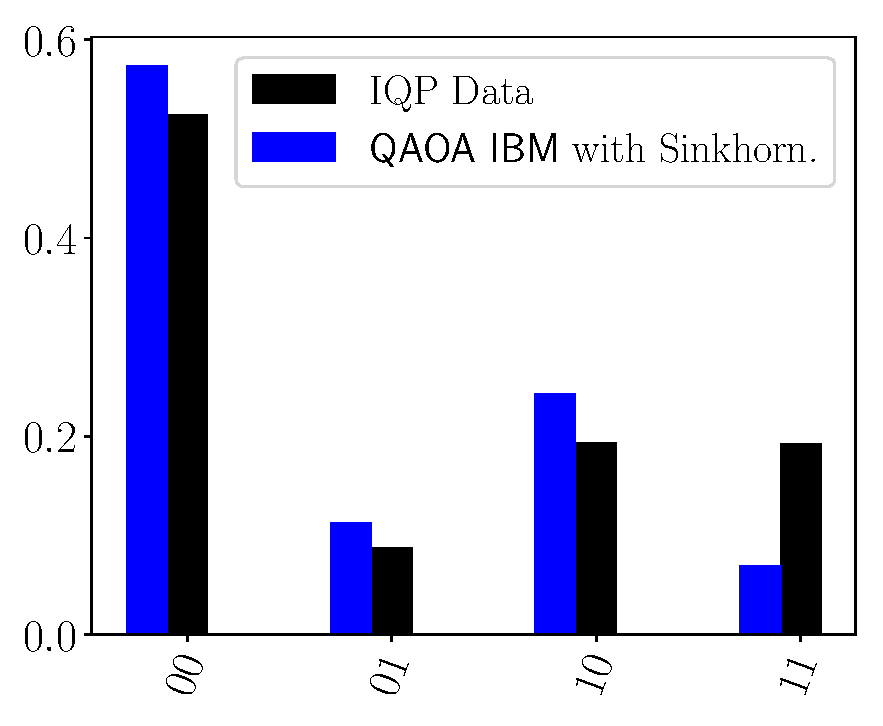
\includegraphics[width=\textwidth, height = 0.8\textwidth]{images/FIG_6b_compilation_probs_2_qubits_qaoa_to_IQP_sinkhorn_eps_0_1_lr_0_05_AVERAGE}};
  \node[below=of img, node distance=0cm, yshift=1.35cm,font=\color{black}] {outcomes};
  \node[left=of img, node distance=0cm, rotate=90, anchor=center,yshift=-0.95cm,font=\color{black}] {probability};
\end{tikzpicture}
    \caption{}
    \label{subfig:auto_comp_final_probs_2}
\end{subfigure}
~
\begin{subfigure}[t]{0.27\textwidth}
        \centering
        % \includegraphics[width=\textwidth, height = 0.8\textwidth]{images/compilation_TV_2_qubits_qaoa_to_IQP_sinkhorn_eps_0_1_lr_0_05_AVERAGE.pdf}
        \begin{tikzpicture}
  \node (img)  {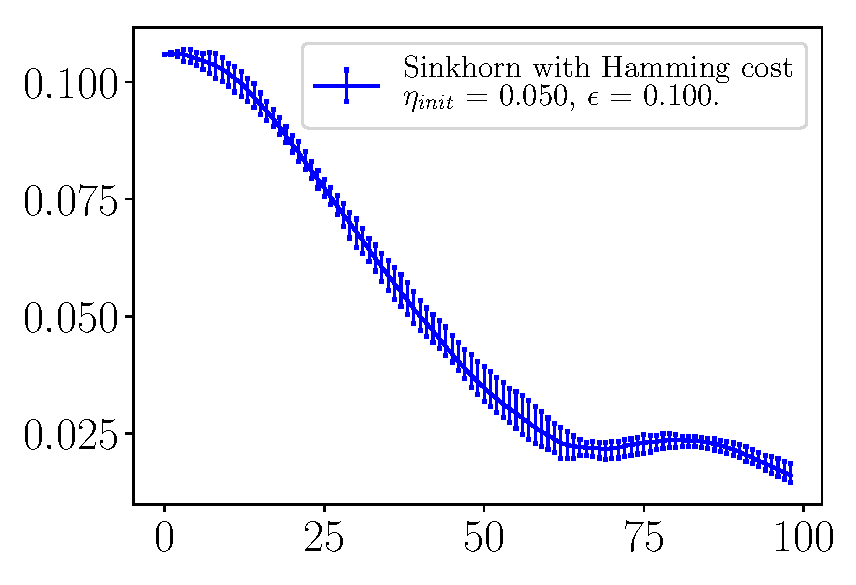
\includegraphics[width=\textwidth, height = 0.8\textwidth]{images/FIG_6c_compilation_TV_2_qubits_qaoa_to_IQP_sinkhorn_eps_0_1_lr_0_05_AVERAGE}};
  \node[below=of img, node distance=0cm, yshift=1.35cm,font=\color{black}] {epoch};
  \node[left=of img, node distance=0cm, rotate=90, anchor=center,yshift=-0.95cm,font=\color{black}] {$\TV$};
\end{tikzpicture}
    \caption{}
    \label{subfig:auto_comp_TV_2}
\end{subfigure}
~
\begin{subfigure}[t]{0.27\textwidth}
        \centering
        % \includegraphics[width=\textwidth, height = 0.8\textwidth]{images/compilation_SINK_2_qubits_qaoa_to_IQP_sinkhorn_eps_0_1_lr_0_05_AVERAGE.pdf}
\begin{tikzpicture}
  \node (img)  {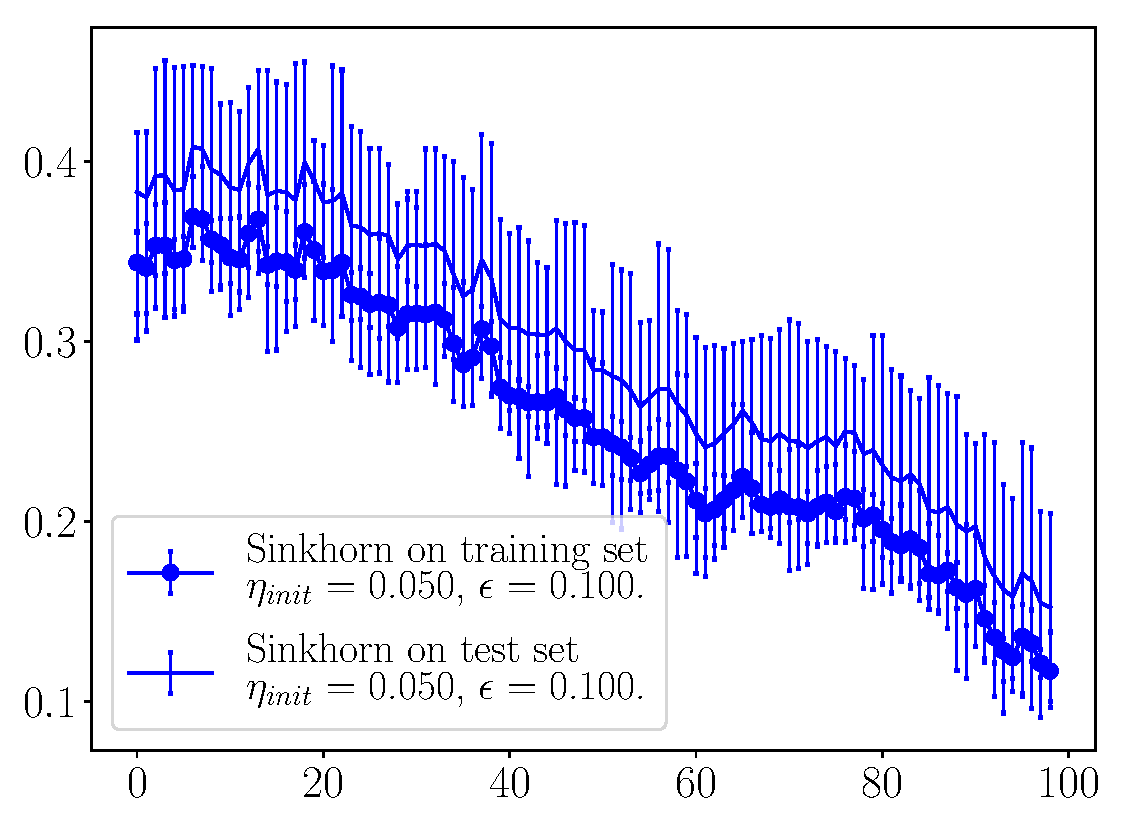
\includegraphics[width=\textwidth, height = 0.8\textwidth]{images/FIG_6d_compilation_SINK_2_qubits_qaoa_to_IQP_sinkhorn_eps_0_1_lr_0_05_AVERAGE}};
  \node[below=of img, node distance=0cm, yshift=1.35cm,font=\color{black}] {epoch};
  \node[left=of img, node distance=0cm, rotate=90, anchor=center,yshift=-0.95cm,font=\color{black}] {$\mathcal{L}_{\SH}$};
\end{tikzpicture}
    \caption{}
    \label{subfig:auto_comp_sink_2_supp}
\end{subfigure}
\caption{Automatic Compilation of $\IQP$ circuit to a $p = 1 \QAOA$ circuit with two qubits using $\mathcal{L}_{\SH}^\epsilon$ with $\epsilon = 0.05$. 1000 data samples were used with 800 used for a training set, and 200 used as a test set. $\IBM$ circuit is able to mimic the target distribution well, even though actual parameter values, and circuit families are different. Error bars represent mean, maximum and minimum values achieved over 5 independent training runs on the same data set. (a) Initial [\crule[cyan]{0.2cm}{0.2cm}] and trained [\crule[Lavender]{0.2cm}{0.2cm}] $\QAOA$ circuit parameters for two qubits. Target $\IQP$ circuit parameters [\crule[green]{0.2cm}{0.2cm}]. Parameter values scaled by a factor of 10 for readability. (b) Final learned probabilities of $\IBM$ ($\QAOA$) [\crule[blue]{0.2cm}{0.2cm}] circuit versus `data' probabilities ($\IQP$) [\crule[black]{0.2cm}{0.2cm}]. (c) Total Variation Distance and (d) Sinkhorn divergence for 800 training samples, 200 test samples, using a Hamming optimal transport cost.}\label{fig:autocompilationtwoqubits}
\end{figure*}



